% Options for packages loaded elsewhere
\PassOptionsToPackage{unicode}{hyperref}
\PassOptionsToPackage{hyphens}{url}
\documentclass[
]{article}
\usepackage{xcolor}
\usepackage{amsmath,amssymb}
\setcounter{secnumdepth}{-\maxdimen} % remove section numbering
\usepackage{iftex}
\ifPDFTeX
  \usepackage[T1]{fontenc}
  \usepackage[utf8]{inputenc}
  \usepackage{textcomp} % provide euro and other symbols
\else % if luatex or xetex
  \usepackage{unicode-math} % this also loads fontspec
  \defaultfontfeatures{Scale=MatchLowercase}
  \defaultfontfeatures[\rmfamily]{Ligatures=TeX,Scale=1}
\fi
\usepackage{lmodern}
\ifPDFTeX\else
  % xetex/luatex font selection
\fi
% Use upquote if available, for straight quotes in verbatim environments
\IfFileExists{upquote.sty}{\usepackage{upquote}}{}
\IfFileExists{microtype.sty}{% use microtype if available
  \usepackage[]{microtype}
  \UseMicrotypeSet[protrusion]{basicmath} % disable protrusion for tt fonts
}{}
\makeatletter
\@ifundefined{KOMAClassName}{% if non-KOMA class
  \IfFileExists{parskip.sty}{%
    \usepackage{parskip}
  }{% else
    \setlength{\parindent}{0pt}
    \setlength{\parskip}{6pt plus 2pt minus 1pt}}
}{% if KOMA class
  \KOMAoptions{parskip=half}}
\makeatother
\usepackage{longtable,booktabs,array}
\newcounter{none} % for unnumbered tables
\usepackage{calc} % for calculating minipage widths
% Correct order of tables after \paragraph or \subparagraph
\usepackage{etoolbox}
\makeatletter
\patchcmd\longtable{\par}{\if@noskipsec\mbox{}\fi\par}{}{}
\makeatother
% Allow footnotes in longtable head/foot
\IfFileExists{footnotehyper.sty}{\usepackage{footnotehyper}}{\usepackage{footnote}}
\makesavenoteenv{longtable}
\usepackage{graphicx}
\makeatletter
\newsavebox\pandoc@box
\newcommand*\pandocbounded[1]{% scales image to fit in text height/width
  \sbox\pandoc@box{#1}%
  \Gscale@div\@tempa{\textheight}{\dimexpr\ht\pandoc@box+\dp\pandoc@box\relax}%
  \Gscale@div\@tempb{\linewidth}{\wd\pandoc@box}%
  \ifdim\@tempb\p@<\@tempa\p@\let\@tempa\@tempb\fi% select the smaller of both
  \ifdim\@tempa\p@<\p@\scalebox{\@tempa}{\usebox\pandoc@box}%
  \else\usebox{\pandoc@box}%
  \fi%
}
% Set default figure placement to htbp
\def\fps@figure{htbp}
\makeatother
\setlength{\emergencystretch}{3em} % prevent overfull lines
\providecommand{\tightlist}{%
  \setlength{\itemsep}{0pt}\setlength{\parskip}{0pt}}
\usepackage{bookmark}
\IfFileExists{xurl.sty}{\usepackage{xurl}}{} % add URL line breaks if available
\urlstyle{same}
\hypersetup{
  hidelinks,
  pdfcreator={LaTeX via pandoc}}

\title{Lie Algebraic Optimization for Continual Learning and Targeted Unlearning in Neural Networks\thanks{Code, data, seeds, and the source of this paper are archived at \href{https://doi.org/10.5281/zenodo.21267659}{doi:10.5281/zenodo.21267659}, mirrored at \url{https://github.com/design-smith/lie-algebraic-unlearning-release}.}}
\author{Nathan Gandawa\\ \texttt{nathan.gandawa@techtorch.io}}
\date{}

\begin{document}

\maketitle

\begin{abstract}

Continual adaptation and targeted unlearning ask a model to change specific behaviors while preserving the rest, and to stay stable when many such changes are applied in sequence. Most parameter-efficient fine-tuning methods adapt weights additively, replacing \(W\) with \(W+\Delta\). Additive parameterizations are order-blind: the composed weight \(W+\Delta_1+\Delta_2\) is the same in either order, so although sequential additive training is order-dependent, that dependence is invisible in the representation. Nothing computable from the increments records it.

This paper reframes sequential adaptation as non-commutative composition of multiplicative orthogonal updates. Each update is a rotation \(W_{\mathrm{new}}=\exp(A)W\) generated by a skew-symmetric \(A\in\mathfrak{so}(n)\), and a sequence composes as a product of exponentials whose interference is governed by the commutators \([A_i,A_j]\). The orthogonal parameterization is the instrument that makes this composition analyzable: since \(\exp(A)^\top\exp(A)=I\), it exactly preserves the column Gram matrix \(W^\top W\), so the weight-geometry invariants are held fixed and any change in behavior is attributable to the rotation itself, the generators and their brackets, rather than to Gram distortion.

We make three contributions. First, a composition analysis: we bound the error of rank-truncated second-order Baker-Campbell-Hausdorff (BCH) accumulation, separating a BCH term controlled by the generator norm from a rank-truncation term controlled by an Eckart-Young tail. Second, a method: an exact low-rank exponential adapter, differentiated through the matrix exponential with no small-angle approximation, with a retain-gradient projection for targeted unlearning and rank-truncated composition for sequences. Third, an invariant-validity analysis that treats the link from parameter-space geometry to behavioral retention as a hypothesis to be tested, not assumed.

Matrix-level and small-network experiments confirm the geometry, with Gram deviation at numerical precision against roughly \(10^{-2}\) for additive updates, and the composition bound, with second-order BCH accumulation \(27\) to \(2200\) times more accurate than naive generator addition across the norms tested. The central hypothesis, that commutator magnitude predicts sequential interference in transformer unlearning, is stated so that it can be refuted; a first test on Llama-3.2-1B supports it, with the normalized commutator predicting cumulative interference across sequential unlearning windows (Spearman \(\rho=0.25\), \(p=2.6\times10^{-3}\), holding within conditions and after controlling for update magnitude, condition, and pair gap), and the full benchmark test through a standard unlearning harness is the empirical question that remains. We do not claim to eliminate catastrophic forgetting or to guarantee semantic preservation: geometry preservation is a parameter-space property, not a functional one.

\emph{Code, configurations, seeds, and raw results are archived at https://doi.org/10.5281/zenodo.21267659 and mirrored at https://github.com/design-smith/lie-algebraic-unlearning-release}

\end{abstract}

\section{Introduction}\label{introduction}

Large language models are adapted after deployment, and rarely just once. New domains are added, stale or harmful behaviors are removed, and specific training influences are unlearned, often as a stream of requests that arrive over time. Each request should change its target behavior while preserving unrelated capabilities, and the requests should not interfere with one another. This last requirement, stability across a sequence of updates, is the one that current methods handle least well, and it is the subject of this paper.

Parameter-efficient fine-tuning (PEFT) freezes most parameters and trains small update modules. LoRA, adapters, and prompt-tuning variants differ in structure but share an additive form: a pretrained weight \(W\) becomes \(W+\Delta\). Additive parameterizations compose commutatively: as a function of the learned increments, \(W+\Delta_1+\Delta_2\) does not depend on their order. Sequential additive training is of course order-dependent, since \(\Delta_2\) is trained at \(W+\Delta_1\), but that dependence lives in the training trajectory, not in the representation. No algebraic object built from the deltas records it, so at the parameterization level it can be neither measured nor regularized. Additive updates also alter the Gram structure of the weight,

\[
(W+\Delta)^\top(W+\Delta)
= W^\top W + W^\top\Delta + \Delta^\top W + \Delta^\top\Delta,
\]

and the cross terms accumulate across a sequence in ways that are hard to attribute to any single task.

We take the opposite starting point. An update is a rotation, \(W_{\mathrm{new}}=\exp(A)W\), generated by a skew-symmetric \(A\in\mathfrak{so}(n)\), and a sequence of updates is the product \(\exp(A_T)\cdots\exp(A_1)\). This composition does not commute, and its non-commutativity is what we want to study: the Baker-Campbell-Hausdorff formula writes the composed generator in terms of the commutators \([A_i,A_j]=A_iA_j-A_jA_i\), which become an explicit, measurable handle on task interference. The orthogonal form is the instrument that makes this clean. Because \(\exp(A)^\top\exp(A)=I\), the transformation preserves the column Gram matrix \(W^\top W\) exactly, so the weight-geometry invariants are held fixed and any change in behavior is attributable to the rotation itself, the generators and their brackets, rather than to Gram distortion.

Two further pieces complete the method. For targeted unlearning, a retain-gradient generator \(S_r\) identifies the skew directions along which an update would perturb retained behavior to first order, and candidate updates are projected onto its orthogonal complement. For scalable sequences, generators are low-rank and the accumulated history is held at a fixed rank by a skew-preserving truncation, with a proven bound on the resulting composition error. We are careful throughout about what the geometry buys: \(\exp(A)W\) preserves parameter-space geometry, not the functional behavior of a nonlinear transformer, so Gram preservation is a controlled invariant to build on, not a guarantee of semantic retention.

The paper makes three contributions.

\begin{enumerate}
\def\labelenumi{\arabic{enumi}.}
\tightlist
\item
  \textbf{Composition analysis.} We formulate sequential adaptation as non-commutative composition on \(SO(n)\) and prove a bound on the error of rank-truncated second-order BCH accumulation, separating a BCH-truncation term (controlled by the generator norm) from a rank-truncation term (an Eckart-Young tail controlled by the retained rank). The second-order BCH term of the bound is confirmed numerically; the rank-truncation term is exercised in the extended matrix study of Section 6.3.
\item
  \textbf{Method.} We give an exact low-rank exponential adapter: the update \(\exp(A)W\) is computed and differentiated exactly, with no small-angle approximation and no Taylor-order hyperparameter; a retain-gradient projection enforces first-order retention; and rank-truncated composition accumulates a sequence of updates within a fixed parameter budget.
\item
  \textbf{Invariant-validity analysis.} We treat the link from parameter-space geometry to behavioral retention as a hypothesis rather than an assumption, and specify how to test whether Gram preservation predicts retention, reporting the result whichever way it falls.
\end{enumerate}

\section{Background and Problem Setup}\label{background-and-problem-setup}

\subsection{Notation}\label{notation}

Let \(W\in\mathbb{R}^{n\times d}\) denote a pretrained weight matrix from a transformer layer. The Lie algebra of the special orthogonal group is

\[
\mathfrak{so}(n)=\{A\in\mathbb{R}^{n\times n}: A^\top=-A\}.
\]

For \(A\in\mathfrak{so}(n)\), the matrix exponential satisfies \(\exp(A)\in SO(n)\), where

\[
SO(n)=\{R\in\mathbb{R}^{n\times n}: R^\top R=I,\ \det(R)=1\}.
\]

The Frobenius inner product is

\[
\langle X,Y\rangle_F=\mathrm{tr}(X^\top Y),
\]

with norm \(\|X\|_F=\sqrt{\langle X,X\rangle_F}\). The Lie bracket of two matrices is

\[
[A,B]=AB-BA.
\]

\subsection{Continual Adaptation and Targeted Unlearning}\label{continual-adaptation-and-targeted-unlearning}

The framework considers a frozen pretrained weight \(W\) and learns a transformation that modifies a target behavior while preserving unrelated behavior. For unlearning, let \(\mathcal{D}_f\) denote a forget set and \(\mathcal{D}_r\) denote a retain set. The forget set contains examples whose influence or behavior should be reduced. The retain set contains examples whose behavior should remain stable.

Let \(L_f(W)\) denote a forget objective and \(L_r(W)\) denote a retain objective. The method optimizes a generator \(A\in\mathfrak{so}(n)\) so that the transformed weight \(\exp(A)W\) reduces the forget objective while constraining first-order damage to retained behavior. A generic constrained formulation is

\[
\min_{A\in\mathfrak{so}(n)} L_f(\exp(A)W)
\]

subject to

\[
\langle A,S_r\rangle_F=0,\qquad \|A\|_F\leq \varepsilon,
\]

where \(S_r\) is the retain-gradient generator defined in Section 3.4 and \(\varepsilon\) bounds the update magnitude.

\subsection{Design Desiderata}\label{design-desiderata}

A geometric adaptation method for continual learning should satisfy four desiderata. First, finite updates should preserve the intended transformation constraint rather than relying only on infinitesimal approximations. Second, the method should distinguish target-change directions from retain-preserving directions. Third, sequential updates should account for the fact that rotations do not generally commute. Fourth, the parameterization should be scalable enough to apply to large model layers.

These desiderata motivate the use of \(\mathfrak{so}(n)\) as the trainable space. Skew-symmetric generators admit exact orthogonal transformations through the exponential map, they form a vector space suitable for projected optimization, their commutator remains inside the same Lie algebra, and low-rank parameterizations can reduce trainable degrees of freedom from \(O(n^2)\) to \(O(nr)\).

\section{Lie Algebraic Constrained Adaptation}\label{lie-algebraic-constrained-adaptation}

\subsection{Overview}\label{overview}

The proposed method adapts a weight matrix by learning a skew-symmetric generator and applying it multiplicatively:

\[
W_{\mathrm{new}}=\exp(A)W,\qquad A\in\mathfrak{so}(n).
\]

The pipeline has four modules. The orthogonal update module maps \(A\) to \(SO(n)\) through the exponential map. The retain-projection module removes first-order directions that would change a retain objective. The stability module bounds the size and numerical drift of the generator. The sequential-composition module uses BCH correction and commutator regularization when multiple tasks are learned or unlearned over time.

\subsection{Orthogonal Update Module}\label{orthogonal-update-module}

The orthogonal update module replaces additive parameter motion with multiplicative transformation motion. Given a pretrained matrix \(W\) and generator \(A\in\mathfrak{so}(n)\), it computes \(R=\exp(A)\) and applies \(W_{\mathrm{new}}=RW\). Since \(A^\top=-A\), the exponential satisfies

\[
R^\top R=\exp(A)^\top\exp(A)=\exp(-A)\exp(A)=I.
\]

This design preserves the column Gram matrix exactly:

\[
W_{\mathrm{new}}^\top W_{\mathrm{new}}
=W^\top R^\top R W
=W^\top W.
\]

The advantage of this module is that the preservation property holds for finite updates. A first-order approximation such as \((I+A)W\) is orthogonal only up to first order because

\[
(I+A)^\top(I+A)=I+A^\top A
\]

for skew-symmetric \(A\). The quadratic term is small only when \(\|A\|\) is small, and it can accumulate across updates.

\subsection{Optimization in the Lie Algebra}\label{optimization-in-the-lie-algebra}

The optimization module computes a candidate update direction in the ambient matrix space and projects it back to \(\mathfrak{so}(n)\). Let

\[
J(A)=L_f(\exp(A)W).
\]

The exact Frechet derivative of the exponential gives

\[
D\exp_A[V]=\int_0^1 \exp((1-\tau)A)V\exp(\tau A)\,d\tau.
\]

If \(G_f=\nabla_{W_{\mathrm{new}}}L_f(W_{\mathrm{new}})\), then the directional derivative satisfies

\[
DJ(A)[V]
=\left\langle G_f, D\exp_A[V]W\right\rangle_F.
\]

The exact gradient follows by taking the adjoint of \(D\exp_A\) under the Frobenius inner product. With the ambient gradient with respect to \(R=\exp(A)\) equal to \(G_fW^\top\),

\[
\nabla_A J = D\exp_A^{*}[G_fW^\top]=D\exp_{A^\top}[G_fW^\top].
\]

This is computed exactly as the top-right \(n\times n\) block of a single \(2n\times 2n\) exponential,

\[
D\exp_{A^\top}[X]=\text{top-right block of }
\exp\begin{pmatrix}A^\top & X\\ 0 & A^\top\end{pmatrix},
\qquad X=G_fW^\top,
\]

or equivalently by automatic differentiation through the matrix exponential. The orthogonal projection of any matrix \(M\) onto \(\mathfrak{so}(n)\) is

\[
P_{\mathfrak{so}}(M)=\frac{1}{2}(M-M^\top),
\]

and the Lie algebra gradient is \(g_A=P_{\mathfrak{so}}(\nabla_A J)\). The small-generator approximation \(D\exp_A[V]\approx V\) recovers the simpler expression \(g_A\approx\frac{1}{2}(G_fW^\top-WG_f^\top)\) in the limit \(\|A\|\to 0\), but its directional error grows with \(\|A\|\), so the method uses the exact gradient. The projection is necessary because unconstrained gradients need not respect skew-symmetry, and the projected direction remains inside the tangent representation used by the exponential map.

\subsection{Retain-Gradient Orthogonality}\label{retain-gradient-orthogonality}

The retain-projection module removes first-order directions that would perturb the retain objective. Let \(G_r=\nabla_W L_r(W)\) be the retain gradient at the pretrained or current retained reference point. For an infinitesimal skew-symmetric update \(W'=(I+A)W\), the first-order retain-loss variation is

\[
\delta L_r=\langle G_r,AW\rangle_F.
\]

Using cyclic trace identities, this variation can be written as an inner product in \(\mathfrak{so}(n)\):

\[
\delta L_r=\langle A,S_r\rangle_F,
\]

where

\[
S_r=\frac{1}{2}(G_rW^\top-WG_r^\top)\in\mathfrak{so}(n).
\]

Therefore, the constraint

\[
\langle A,S_r\rangle_F=0
\]

is a condition for first-order retain invariance. With a normalized retain basis \(\{\widehat{S}_{r,i}\}_{i=1}^m\), the projected forget direction is

\[
g_{\mathrm{null}}
=g_A-\sum_{i=1}^{m}\langle g_A,\widehat{S}_{r,i}\rangle_F\widehat{S}_{r,i}.
\]

In practice, the retain subspace can be estimated from minibatches, task gradients, or low-rank sketches of retain gradients. If only one retain direction is used, the projection reduces to

\[
g_{\mathrm{null}}
=g_A-
\frac{\langle g_A,S_r\rangle_F}{\|S_r\|_F^2+\xi}S_r,
\]

where \(\xi>0\) is a numerical stabilizer.

The retain generator must not go stale. Estimating \(S_r\) once at a single reference point is insufficient under finite and sequential updates, because the retain gradient drifts as \(W_{\mathrm{new}}\) moves and as later tasks arrive. Within a task, the framework refreshes the retain basis every \(k\) steps at the current \(W_{\mathrm{new}}\): it draws \(B\) retain minibatches, forms the corresponding generators \(S_r^{(b)}\), and keeps a Frobenius-orthonormal basis capturing an energy fraction \(\rho_E\) of the stacked generators. Across tasks, it maintains a growing gradient-projection memory: after each task the new retain directions are orthogonalized against the existing memory and the residual directions are appended, so directions the model was asked to protect earlier stay protected as new unlearning requests arrive. Every update projects onto the orthogonal complement of the current memory.

This estimator has two failure modes. If the subspace under-covers the true retain-sensitive directions, because the energy threshold is too low, the refresh too infrequent, or the memory cap too small, those directions are left unprotected and retained behavior degrades. If it over-covers, absorbing directions that also carry the forget signal, then projecting them out weakens unlearning. The energy fraction \(\rho_E\) sets the operating point between these two, and the forget-retain trade-off is where its choice is judged.

The guarantee of Proposition 2 attaches to the applied update, not merely to the gradient. An optimizer that preconditions per coordinate, such as Adam, maps a null-space gradient to an update with components along the retain directions, and momentum accumulates the violation. Projected variants therefore use plain projected gradient steps, or equivalently apply the projection to the optimizer's composed update immediately before it reaches the parameters.

\subsection{Stability and Norm Control}\label{stability-and-norm-control}

The stability module bounds the generator so that the exponential approximation and BCH truncation remain in a controlled regime. A simple regularized objective is

\[
\widetilde{J}(A)=L_f(\exp(A)W)+\lambda_{\mathrm{stab}}\|A\|_F^2.
\]

The corresponding stability gradient is

\[
g_{\mathrm{stab}}=2\lambda_{\mathrm{stab}}A.
\]

After each update, the generator can be projected onto a Frobenius ball:

\[
A\leftarrow
\begin{cases}
A, & \|A\|_F\leq \varepsilon,\\
\varepsilon A/\|A\|_F, & \|A\|_F>\varepsilon.
\end{cases}
\]

Finally, numerical roundoff can introduce small symmetric components. The method restores structural validity with

\[
A\leftarrow \frac{1}{2}(A-A^\top).
\]

\subsection{Low-Rank Skew-Symmetric Parameterization}\label{low-rank-skew-symmetric-parameterization}

Full skew-symmetric matrices require \(n(n-1)/2\) degrees of freedom, which is too large for many transformer layers. The method therefore admits a low-rank generator

\[
A=UV^\top-VU^\top,\qquad U,V\in\mathbb{R}^{n\times r}.
\]

This form guarantees \(A^\top=-A\) while using \(2nr\) trainable parameters. Its rank satisfies

\[
\mathrm{rank}(A)\leq 2r.
\]

The trade-off is explicit: smaller \(r\) improves efficiency but restricts the accessible rotation directions. In continual learning, this restriction can be interpreted as a limited budget of Lie algebra directions that must be allocated across tasks. The rank bound \(\mathrm{rank}(A)\leq 2r\) holds for a single task's generator. It does not carry over to the accumulated history under sequential composition, because commutators raise rank; Section 3.8 handles the accumulated object separately.

\subsection{Matrix-Free Exponential Action}\label{matrix-free-exponential-action}

For large layers, explicitly forming \(\exp(A)\) is unnecessary: the framework only needs the action of \(\exp(A)\) on activations or weight outputs, and the low-rank structure makes that action exact and cheap. Write the low-rank generator as \(A=UV^\top-VU^\top=[U\ V]\,J\,[U\ V]^\top\) with

\[
J=\begin{pmatrix}0 & I_r\\ -I_r & 0\end{pmatrix}\in\mathbb{R}^{2r\times 2r}.
\]

Take the thin QR factorization \([U\ V]=Q\check{R}\) with \(Q\in\mathbb{R}^{n\times 2r}\), \(Q^\top Q=I_{2r}\), and set \(M=\check{R}J\check{R}^\top\in\mathbb{R}^{2r\times 2r}\). Then \(M\) is skew-symmetric and \(A=QMQ^\top\), so \(A^k=QM^kQ^\top\) for \(k\ge 1\) and

\[
\exp(A)=I+Q\big(\exp(M)-I\big)Q^\top,\qquad
\exp(A)\,x=x+Q\big(\exp(M)-I\big)\big(Q^\top x\big).
\]

Here \(\exp(M)\) is a dense \(2r\times 2r\) exponential, computed exactly. The action costs \(O(nr)\) per input plus one small \(O((2r)^3)\) exponential per update, and never forms a dense \(n\times n\) matrix. Because it is exact, it removes the truncation order that a Taylor-series action would require. The same construction applies to the rank-\(2R\) accumulated history of Section 3.8: the truncation returns it in the factored form \(\tilde{H}=Z\Theta Z^\top\) with \(Z^\top Z=I_{2R}\), so \(\exp(\tilde{H})=I+Z(\exp(\Theta)-I)Z^\top\) at cost \(O(nR)\).

\subsection{BCH-Aware Sequential Composition}\label{bch-aware-sequential-composition}

Sequential adaptation is not additive when updates are multiplicative. For two tasks with generators \(A_1,A_2\in\mathfrak{so}(n)\),

\[
\exp(A_2)\exp(A_1)\neq \exp(A_1+A_2)
\]

in general. The correct composed generator is

\[
A_{\mathrm{total}}
=\log(\exp(A_2)\exp(A_1)).
\]

The BCH expansion gives

\[
A_{\mathrm{total}}
=A_1+A_2+\frac{1}{2}[A_2,A_1]+O(\|A\|^3),
\]

where \(\|A\|=\max(\|A_1\|,\|A_2\|)\). For an accumulated history \(A_{\mathrm{hist}}\) and a new update \(A\), the second-order accumulation rule is

\[
A_{\mathrm{hist}}\leftarrow
A_{\mathrm{hist}}+A+\frac{1}{2}[A,A_{\mathrm{hist}}].
\]

This correction makes order-dependent interference explicit in the second-order approximation. If two generators commute, then \([A_i,A_j]=0\) and the second-order interaction vanishes. If the commutator is large, the two updates interact strongly under composition.

The accumulation rule creates a tension with the low-rank parameterization of Section 3.6. Each per-task generator has rank at most \(2r\), but the commutator \([A,A_{\mathrm{hist}}]\) can have rank up to \(4r\), so naively summing generators across tasks raises the rank of the history and eventually destroys the low-rank structure that made the method scalable. The framework resolves this by maintaining the history at a fixed rank budget \(2R\): after each accumulation step it applies a skew-preserving best rank-\(2R\) truncation,

\[
\tilde{H}_t=\mathcal{T}_{2R}\!\left(\tilde{H}_{t-1}+A_t+\tfrac{1}{2}[A_t,\tilde{H}_{t-1}]\right),
\]

where \(\mathcal{T}_{2R}\) keeps the \(R\) largest \(2\times 2\) blocks of the real Schur form and remains inside \(\mathfrak{so}(n)\). Theorem 1 (Section 4) bounds the resulting composition error and separates it into a second-order BCH term, controlled by the generator norms, and a rank-truncation term, controlled by the budget \(R\). When exact composition is required instead, the ordered generators \(\{A_t\}\) can be stored and applied as the product \(\exp(A_T)\cdots\exp(A_1)\), which is exact at the cost of application linear in the number of tasks.

\subsection{Commutator Regularization}\label{commutator-regularization}

The commutator regularization module discourages new updates from strongly interfering with the accumulated history. Define

\[
L_{\mathrm{BCH}}(A)=\|[A,A_{\mathrm{hist}}]\|_F^2.
\]

Let

\[
C=[A,A_{\mathrm{hist}}]=AA_{\mathrm{hist}}-A_{\mathrm{hist}}A.
\]

For skew-symmetric \(A_{\mathrm{hist}}\), the gradient is

\[
\nabla_A L_{\mathrm{BCH}}
=2(A_{\mathrm{hist}}C-CA_{\mathrm{hist}}).
\]

The total update direction is

\[
g_{\mathrm{total}}
=g_{\mathrm{null}}+g_{\mathrm{stab}}
+\lambda_{\mathrm{BCH}}\nabla_A L_{\mathrm{BCH}}.
\]

This term does not guarantee compatibility among tasks, but it supplies a direct geometric penalty for non-commuting updates.

\subsection{Algorithm}\label{algorithm}

\textbf{Algorithm 1: Lie Algebraic Constrained Update with BCH-Aware Composition}

\textbf{Input:} pretrained weight \(W\), forget data \(\mathcal{D}_f\), retain data or retain gradient estimate \(\mathcal{D}_r\), learning rate \(\eta\), stability coefficient \(\lambda_{\mathrm{stab}}\), BCH coefficient \(\lambda_{\mathrm{BCH}}\), norm bound \(\varepsilon\), history norm bound \(\rho_{\max}\), per-task rank \(r\), truncation rank \(R\), retain energy fraction \(\rho_E\), refresh period \(k\).

\textbf{Initialize:} \(A\leftarrow 0\), \(A_{\mathrm{hist}}\leftarrow 0\).

\begin{enumerate}
\def\labelenumi{\arabic{enumi}.}
\tightlist
\item
  Estimate the retain basis \(\{\widehat{S}_{r,i}\}\) from \(\mathcal{D}_r\) at the current weight (Section 3.4), retaining energy fraction \(\rho_E\).
\item
  For each forget minibatch, apply \(W_{\mathrm{new}}=\exp(A)W\) through the exact low-rank action of Section 3.7.
\item
  Compute the forget gradient \(G_f\) at the transformed output.
\item
  Compute the exact gradient \(\nabla_A J=D\exp_{A^\top}[G_fW^\top]\) (Section 3.3) and project it into the Lie algebra: \(g_A=P_{\mathfrak{so}}(\nabla_A J)\).
\item
  Project away retain directions: \(g_{\mathrm{null}}=g_A-\sum_i\langle g_A,\widehat{S}_{r,i}\rangle_F\widehat{S}_{r,i}\); refresh the basis every \(k\) steps.
\item
  Add stability and commutator terms:
\end{enumerate}

\[
g_{\mathrm{total}}
=g_{\mathrm{null}}+2\lambda_{\mathrm{stab}}A
+\lambda_{\mathrm{BCH}}\nabla_A\|[A,A_{\mathrm{hist}}]\|_F^2.
\]

\begin{enumerate}
\def\labelenumi{\arabic{enumi}.}
\setcounter{enumi}{6}
\tightlist
\item
  Update \(A\leftarrow A-\eta g_{\mathrm{total}}\) (plain gradient step; if an adaptive optimizer is used, project its composed update instead).
\item
  Project \(A\) to the Frobenius ball and restore skew-symmetry with \(A\leftarrow\frac{1}{2}(A-A^\top)\).
\item
  After completing the task, accumulate the history with rank-\(2R\) truncation, then restore skew-symmetry and bound its norm, and append the task's retain directions to the projection memory:
\end{enumerate}

\[
A_{\mathrm{hist}}\leftarrow
\mathcal{T}_{2R}\!\left(A_{\mathrm{hist}}+A+\frac{1}{2}[A,A_{\mathrm{hist}}]\right),
\qquad
A_{\mathrm{hist}}\leftarrow \Pi_{\rho_{\max}}(A_{\mathrm{hist}}),
\]

where \(\mathcal{T}_{2R}\) is the skew-preserving rank-\(2R\) truncation of Section 3.8 and \(\Pi_{\rho_{\max}}\) restores skew-symmetry and projects onto the Frobenius ball of radius \(\rho_{\max}\), chosen so \(\varepsilon+\rho_{\max}<\ln 2\). Log the clip displacement \(\kappa=\|\breve{A}-\Pi_{\rho_{\max}}(\breve{A})\|_F\), where \(\breve{A}=\mathcal{T}_{2R}(A_{\mathrm{hist}}+A+\tfrac{1}{2}[A,A_{\mathrm{hist}}])\), so a run can report whether it ever left the active regime of Theorem 1 (\(\kappa>0\)).

\textbf{Output:} accumulated generator \(A_{\mathrm{hist}}\) and transformed weight \(W_{\mathrm{final}}=\exp(A_{\mathrm{hist}})W\).

\subsection{Transformer Placement}\label{transformer-placement}

The adapter is applied by left multiplication, \(W_{\mathrm{new}}=\exp(A)W\) with \(A\in\mathfrak{so}(d_{\mathrm{out}})\), which preserves the column Gram matrix \(W^\top W\) (Proposition 1). The primary targets are the residual-stream write matrices, attention \(o_{\mathrm{proj}}\) and MLP \(\mathrm{down}_{\mathrm{proj}}\), both of which have \(d_{\mathrm{out}}=d_{\mathrm{model}}\). Placing the adapter there keeps every generator in a single \(\mathfrak{so}(d_{\mathrm{model}})\), so sequential composition and commutator interference are measured in one Lie algebra across layers and tasks. The query, key, value, gate, and up projections are ablation targets; for the head-structured \(q\), \(k\), and \(v\) projections the generator is block-diagonal, one \(\mathfrak{so}(d_{\mathrm{head}})\) block per head, so that rotations do not mix heads.

At a matched trainable-parameter budget the adapter is competitive with additive and orthogonal baselines. On Llama-3.2-1B, adapting \(o_{\mathrm{proj}}\) and \(\mathrm{down}_{\mathrm{proj}}\) across all layers at rank \(r\) uses \(2r\,d_{\mathrm{model}}\) parameters per matrix. Matching the trainable budget of a rank-8 LoRA on the same matrices, about \(1.84\) million parameters or \(0.11\%\) of the model's linear-layer parameters, corresponds to \(r=14\). The exact low-rank action costs \(O(d_{\mathrm{model}}\,r)\) per token, the same order as LoRA, and lower than LoRA on the wide \(\mathrm{down}_{\mathrm{proj}}\) because the cost scales with \(d_{\mathrm{out}}\) alone rather than \(d_{\mathrm{out}}+d_{\mathrm{in}}\).

\section{Theoretical Guarantees}\label{theoretical-guarantees}

\subsection{Proposition 1: Orthogonal Updates Preserve the Gram Matrix}\label{proposition-1-orthogonal-updates-preserve-the-gram-matrix}

Let \(W\in\mathbb{R}^{n\times d}\) and \(A\in\mathfrak{so}(n)\). Define \(W_{\mathrm{new}}=\exp(A)W\). Then

\[
W_{\mathrm{new}}^\top W_{\mathrm{new}}=W^\top W.
\]

\textbf{Proof.} Since \(A^\top=-A\), \(\exp(A)^\top=\exp(-A)\). Therefore \(\exp(A)^\top\exp(A)=\exp(-A)\exp(A)=I\). Hence

\[
W_{\mathrm{new}}^\top W_{\mathrm{new}}
=W^\top\exp(A)^\top\exp(A)W
=W^\top W.
\]

This proves the claim at the transformed weight level. \(\square\)

\subsection{Proposition 2: Retain-Gradient Orthogonality Gives First-Order Retain Invariance}\label{proposition-2-retain-gradient-orthogonality-gives-first-order-retain-invariance}

Let \(L_r(W)\) be a retain loss with gradient \(G_r=\nabla_W L_r(W)\). Define

\[
S_r=\frac{1}{2}(G_rW^\top-WG_r^\top).
\]

For an infinitesimal update \(W'=(I+A)W\) with \(A\in\mathfrak{so}(n)\), if \(\langle A,S_r\rangle_F=0\), then \(\delta L_r=0\) to first order.

\textbf{Proof.} The first-order variation is

\[
\delta L_r=\langle G_r,AW\rangle_F
=\mathrm{tr}(G_r^\top AW).
\]

By cyclic trace invariance,

\[
\delta L_r=\mathrm{tr}(AWG_r^\top).
\]

Only the skew-symmetric component of \(G_rW^\top\) contributes when paired with \(A\in\mathfrak{so}(n)\). That skew component is \(S_r\). Therefore

\[
\delta L_r=\langle A,S_r\rangle_F.
\]

If \(\langle A,S_r\rangle_F=0\), the first-order retain variation is zero. \(\square\)

\subsection{Background Lemmas}\label{background-lemmas}

Three classical facts about \(\mathfrak{so}(n)\) are used above and stated here without proof (see Hall, 2015; Gallier and Quaintance, 2020). First, the Lie algebra is closed under the commutator: for \(A,B\in\mathfrak{so}(n)\), \([A,B]=AB-BA\in\mathfrak{so}(n)\), since \([A,B]^\top=B^\top A^\top-A^\top B^\top=BA-AB=-[A,B]\). Second, the Baker-Campbell-Hausdorff expansion is

\[
\log(\exp(X)\exp(Y))
=X+Y+\tfrac{1}{2}[X,Y]
+\tfrac{1}{12}[X,[X,Y]]
-\tfrac{1}{12}[Y,[X,Y]]+\cdots,
\]

and truncating it after the second-order term gives the accumulation rule of Section 3.8, whose error Theorem 1 bounds. Third, \(\dim\mathfrak{so}(n)=n(n-1)/2\), since a skew-symmetric matrix is fixed by its \(\binom{n}{2}\) strictly-upper-triangular entries. These are background. The load-bearing results are Proposition 1 (Gram preservation), Proposition 2 (first-order retain invariance), Proposition 6 (low-rank capacity), and Theorem 1 (the composition error bound); each is elementary, and the work is in how they combine and in the empirical tests.

\subsection{Proposition 6: Low-Rank Generators Have Bounded Rank and Parameter Count}\label{proposition-6-low-rank-generators-have-bounded-rank-and-parameter-count}

Let \(A=UV^\top-VU^\top\) with \(U,V\in\mathbb{R}^{n\times r}\). Then \(A\in\mathfrak{so}(n)\), \(\mathrm{rank}(A)\leq 2r\), and the parameter count is \(2nr\) before accounting for non-identifiability.

\textbf{Proof.} The transpose satisfies

\[
A^\top=(UV^\top-VU^\top)^\top=VU^\top-UV^\top=-A,
\]

so \(A\) is skew-symmetric. Since \(\mathrm{rank}(UV^\top)\leq r\) and \(\mathrm{rank}(VU^\top)\leq r\),

\[
\mathrm{rank}(A)\leq \mathrm{rank}(UV^\top)+\mathrm{rank}(VU^\top)\leq 2r.
\]

The matrices \(U\) and \(V\) contain \(2nr\) scalar parameters. \(\square\)

\subsection{Theorem 1: Composition Error under Rank-Truncated Accumulation}\label{theorem-1-composition-error-under-rank-truncated-accumulation}

The low-rank parameterization of Section 3.6 and the accumulation rule of Section 3.8 are in tension: the commutator of two rank-\(\leq 2r\) skew matrices can have rank up to \(4r\), so repeated accumulation raises the rank of the history without bound. The method holds the history at a fixed rank budget \(2R\) through a skew-preserving truncation, and the following result bounds the cost of doing so. It is the paper's central composition guarantee.

Let \(\mathcal{T}_{2R}\) denote best rank-\(2R\) Frobenius approximation restricted to \(\mathfrak{so}(n)\). For skew \(B\) with real Schur angles \(\theta_1\geq\theta_2\geq\cdots\geq 0\), it keeps the \(R\) largest \(2\times 2\) blocks, with ties among equal angles broken by retaining conjugate blocks whole, remains skew-symmetric, and satisfies the Eckart-Young identity

\[
\|B-\mathcal{T}_{2R}(B)\|_F=\sqrt{\sum_{i>2R}\sigma_i(B)^2}.
\]

Given per-task generators \(A_1,\dots,A_T\in\mathfrak{so}(n)\) with \(\|A_t\|_F\leq\varepsilon\), define the truncated accumulation \(\tilde{H}_0=0\), \(\hat{B}_t=\tilde{H}_{t-1}+A_t+\tfrac{1}{2}[A_t,\tilde{H}_{t-1}]\), \(\breve{B}_t=\mathcal{T}_{2R}(\hat{B}_t)\), and \(\tilde{H}_t=\Pi_{\rho_{\max}}(\breve{B}_t)\), where \(\Pi_{\rho_{\max}}\) is the Frobenius-ball clip of Algorithm 1; set \(\tilde{R}_T=\exp(\tilde{H}_T)\). Let \(R_{\mathrm{exact}}=\exp(A_T)\cdots\exp(A_1)\) be the exact composed transformation.

\textbf{Theorem 1.} Suppose \(\|H_t\|_F\leq\rho\) and \(\|\tilde{H}_t\|_F\leq\rho\) for all \(t\), with \(\varepsilon+\rho<\ln 2\). Then

\[
\|R_{\mathrm{exact}}-\tilde{R}_T\|_F\leq\sum_{t=1}^{T}L^{\,T-t}\big(\beta_t+\tau_t+\kappa_t\big),
\]

where \(\tau_t=\|\hat{B}_t-\breve{B}_t\|_F=\sqrt{\sum_{i>2R}\sigma_i(\hat{B}_t)^2}\) is the Eckart-Young truncation tail, \(\kappa_t=\|\breve{B}_t-\Pi_{\rho_{\max}}(\breve{B}_t)\|_F\) is the clipping displacement (zero whenever the clip is inactive), the second-order BCH remainder satisfies \(\beta_t\leq\tfrac{1}{3}\varepsilon\rho(\varepsilon+\rho)+C_3(\varepsilon+\rho)^4\), and \(L=(2-e^{\varepsilon+\rho})^{-1}\). The constants \(L\), \(\beta_t\), and \(C_3\) are derived explicitly in Appendix B. In the small-angle regime \(L\to 1\),

\[
\|R_{\mathrm{exact}}-\tilde{R}_T\|_F\leq\frac{T}{3}\varepsilon\rho(\varepsilon+\rho)+\sum_{t=1}^{T}\big(\tau_t+\kappa_t\big)+O\!\big(T(\varepsilon+\rho)^4\big).
\]

\textbf{Proof.} The argument rests on three facts. First, for skew \(X,Y\), \(\|[X,Y]\|_F\leq 2\|X\|_F\|Y\|_F\), since \(\|XY-YX\|_F\leq\|X\|_2\|Y\|_F+\|Y\|_2\|X\|_F\leq 2\|X\|_F\|Y\|_F\). Second, the exponential is \(1\)-Lipschitz on \(\mathfrak{so}(n)\) in Frobenius norm: from \(D\exp_Z[V]=\int_0^1\exp((1-\tau)Z)V\exp(\tau Z)\,d\tau\) with \(Z\) skew, each \(\exp(sZ)\) is orthogonal, so \(\|D\exp_Z[V]\|_F\leq\|V\|_F\), and integrating along the segment between two skew matrices gives \(\|\exp(X)-\exp(Y)\|_F\leq\|X-Y\|_F\). Third, \(\mathcal{T}_{2R}\) attains the Eckart-Young tail and keeps \(\tilde{H}_t\) skew, so the second fact applies to it.

Write \(H_t=\log(\exp(A_t)\exp(H_{t-1}))\), so \(\exp(H_T)=R_{\mathrm{exact}}\), and let \(e_t=\|H_t-\tilde{H}_t\|_F\). The second fact gives \(\|R_{\mathrm{exact}}-\tilde{R}_T\|_F\leq e_T\). Both endpoints of the segment joining \(H_{t-1}\) and \(\tilde{H}_{t-1}\) lie in the ball of radius \(\rho\) by hypothesis, so \(\Phi_{A_t}\) is well defined on it and Lemma B.4 applies. At each step, compare the exact update \(\Phi_{A_t}(X)=\log(\exp(A_t)\exp(X))\) with the truncated second-order update, inserting the untruncated intermediate \(\hat{B}_t=A_t+\tilde{H}_{t-1}+\tfrac{1}{2}[A_t,\tilde{H}_{t-1}]\):

\[
e_t\leq\underbrace{\|\Phi_{A_t}(H_{t-1})-\Phi_{A_t}(\tilde{H}_{t-1})\|_F}_{\leq\, L\,e_{t-1}}+\underbrace{\|\Phi_{A_t}(\tilde{H}_{t-1})-\hat{B}_t\|_F}_{\leq\,\beta_t}+\underbrace{\|\hat{B}_t-\breve{B}_t\|_F}_{=\,\tau_t}+\underbrace{\|\breve{B}_t-\tilde{H}_t\|_F}_{=\,\kappa_t}.
\]

Here \(L=(2-e^{\varepsilon+\rho})^{-1}\) is the Lipschitz constant of \(\Phi_{A_t}\) on the norm ball (Appendix B, Lemma B.4); \(\beta_t\) bounds the dropped third- and higher-order BCH terms (Lemma B.5); \(\tau_t\) is the Eckart-Young truncation tail (Lemma B.3); and \(\kappa_t\) is the clip displacement, which by the \(1\)-Lipschitz property of \(\exp\) enters the transformation error one to one. Unrolling \(e_t\leq L\,e_{t-1}+\beta_t+\tau_t+\kappa_t\) from \(e_0=0\) yields the stated bound, and setting \(L=1\) gives the small-angle form. \(\square\)

The two error sources are controlled independently: the norms \(\varepsilon,\rho\) shrink the BCH term cubically, and the rank budget \(R\) shrinks the truncation term, with \(\tau_t\to 0\) once \(2R\) reaches the rank of \(\hat{B}_t\). Choosing \(R\) so the discarded skew-eigenvalue tail sits below the BCH term makes truncation negligible without going full-rank. When exact composition is required, storing the ordered generators and applying \(\exp(A_T)\cdots\exp(A_1)\) forces every \(\tau_t=\kappa_t=0\), at the cost of application linear in \(T\). A lemma-by-lemma proof with explicit constants is given in Appendix B.

\textbf{Remark (regime of validity).} With \(L=(2-e^{\varepsilon+\rho})^{-1}=1+c(\varepsilon+\rho)\) for a modest \(c\), the prefactors compound to at most \(e^{cT(\varepsilon+\rho)}\), so the bound is informative in the regime \(T(\varepsilon+\rho)=O(1)\). Independently, each task adds at most about \(\varepsilon(1+\rho)\) to the history norm before truncation, so the hypothesis \(\|\tilde{H}_t\|_F\leq\rho\) with \(\varepsilon+\rho<\ln 2\) is sustainable for roughly \(T\lesssim\rho/\varepsilon\) tasks before \(\Pi_{\rho_{\max}}\) activates; for example \(\varepsilon=0.05\) and \(\rho=0.6\) admits on the order of a dozen requests. Beyond this regime the recommended mode is exact product composition (Section 3.8), which stores the ordered generators and forces every \(\tau_t=\kappa_t=0\) at application cost linear in \(T\).

\section{Related Work}\label{related-work}

The framework sits at the intersection of six lines of work. Table 2 summarizes how it is positioned against each.

\subsection{Orthogonal and Lie-group parameterizations}\label{orthogonal-and-lie-group-parameterizations}

Optimizing under orthogonality constraints has a long history in manifold optimization and recurrent networks. Absil, Mahony, and Sepulchre (2008) give the general theory of optimization on matrix manifolds, including the Stiefel and orthogonal groups. For recurrent networks, orthogonal and unitary recurrences were introduced to control gradient norms: Arjovsky, Shah, and Bengio (2016) use unitary evolution, Mhammedi et al.~(2017) use Householder reflections, and Helfrich, Willmott, and Ye (2018) use a scaled Cayley transform. Closest to our parameterization, Lezcano-Casado and Martinez-Rubio (2019) optimize orthogonal and unitary weights directly through the exponential map, and Lezcano-Casado (2019) extends this to trivializations on general matrix manifolds with an explicit formula for the gradient of the matrix exponential. We use the same exponential retraction, but as the substrate for sequential composition and unlearning rather than for training a single constrained weight.

\subsection{Orthogonal parameter-efficient fine-tuning}\label{orthogonal-parameter-efficient-fine-tuning}

Within PEFT, orthogonal transformations were brought to large pretrained models by OFT (Qiu et al., 2023), which adapts weights by a learned rotation to preserve hyperspherical energy in text-to-image diffusion, and BOFT (Liu et al., 2024), which improves parameter efficiency with a butterfly factorization. HRA (Yuan et al., 2024) spans low-rank and orthogonal adaptation with a chain of learnable Householder reflections. These methods motivate the geometric value of rotational adaptation. They differ from the present work in three ways: they typically use Cayley or structured parameterizations rather than explicit exponential-map optimization, they do not impose a retain-objective constraint, and they treat a single transformation rather than the non-commutative composition of a sequence. The dominant PEFT family remains additive: LoRA (Hu et al., 2022) and successors such as QLoRA (Dettmers et al., 2023) and DoRA (Liu et al., 2024), together with adapters (Houlsby et al., 2019), prefix-tuning (Li and Liang, 2021), and prompt tuning (Lester et al., 2021). The first-order rotational update \(W'=(I+A)W\) is only the linear approximation to \(\exp(A)W\) and is treated as such here.

\subsection{Gradient-projection continual learning}\label{gradient-projection-continual-learning}

The retain-gradient projection is closest to gradient-projection methods for continual learning, which avoid disturbing earlier tasks by confining updates to a subspace. Orthogonal Gradient Descent (Farajtabar et al., 2020) projects new-task gradients away from directions that change previous-task outputs; Gradient Projection Memory (Saha, Garg, and Roy, 2021) stores a basis of important past directions and updates in its orthogonal complement; and null-space training (Wang et al., 2021) confines updates to the null space of prior activations. Regularization-based approaches such as EWC (Kirkpatrick et al., 2017) and replay-based methods such as GEM and A-GEM (Lopez-Paz and Ranzato, 2017; Chaudhry et al., 2019) address the same forgetting problem differently. Our retain memory keeps the projection idea but places it inside the Lie algebra: the protected directions are skew generators \(S_r\), and updates are projected in \(\mathfrak{so}(n)\).

\subsection{Machine unlearning methods}\label{machine-unlearning-methods}

Unlearning for language models spans exact and approximate methods. Exact approaches such as SISA (Bourtoule et al., 2021) retrain data shards. Approximate approaches edit a trained model in place: gradient-ascent and gradient-difference objectives raise the loss on a forget set (Jang et al., 2023); NPO (Zhang et al., 2024) recasts this as a preference objective to avoid catastrophic collapse; RMU (Li et al., 2024) redirects the internal representations of forget data; refusal-style baselines map forget queries to ``I do not know''; and Eldan and Russinovich (2023) unlearn a target corpus by fine-tuning on generic relabelings. These define the objectives our adapter optimizes. The contribution here is the update geometry and its composition, not a new forget loss. In unlearning specifically, FALCON (Hu et al., 2025) resolves forget-retain gradient conflicts by projecting them onto orthogonal subspaces; its projection acts on Euclidean parameter and representation gradients, whereas ours acts on skew generators in \(\mathfrak{so}(n)\), which is what lets the projected update compose multiplicatively across a sequence.

\subsection{Sequential and successive unlearning}\label{sequential-and-successive-unlearning}

Most unlearning work studies a single request; the sequential case, where requests arrive over time and can interfere, has only recently received direct treatment. MUSE (Shi et al., 2024) lists sustainability under successive requests among six desiderata and reports that existing methods degrade under repeated removal. O3 (Gao et al., 2024) addresses the same regime by training one LoRA per request and penalizing overlap between successive LoRA subspaces with an orthogonality regularizer. Our approach differs in mechanism and in what it can state: all edits live in a single Lie algebra, order dependence is carried by commutators rather than suppressed by regularization alone, and the accumulated history carries a composition-error bound (Theorem 1). The approaches are complementary; per-request isolation and commutator-aware accumulation could be combined.

\subsection{Benchmarks and critiques}\label{benchmarks-and-critiques}

Evaluating unlearning is itself contested. TOFU (Maini et al., 2024) provides a fictitious-author benchmark with matched forget and retain sets; WMDP (Li et al., 2024) measures hazardous knowledge and its removal; MUSE (Shi et al., 2024) scores six properties including privacy leakage and sequential sustainability. Critiques show that apparent forgetting can hide extractable knowledge or collapse under relearning: Liu et al.~(2024) rethink the problem formulation, and Lynch et al.~(2024) find that different evaluation methods disagree and that unlearned content can be made to resurface. We adopt these benchmarks and metrics rather than proposing new ones.

\subsection{The additive foil: task arithmetic}\label{the-additive-foil-task-arithmetic}

The clearest additive counterpart to our multiplicative view is task arithmetic (Ilharco et al., 2023), which represents a fine-tuned capability as a task vector \(\tau=\theta_{\mathrm{ft}}-\theta_0\) and edits models by adding or subtracting task vectors, including subtraction for forgetting. Merging methods such as model soups (Wortsman et al., 2022) and Ties-Merging (Yadav et al., 2023) extend this additive algebra. Task arithmetic is commutative by construction, \(\tau_1+\tau_2=\tau_2+\tau_1\), so the order of edits is invisible to it. That is exactly the property our framework trades away to gain a model of interference: the commutator \([A_i,A_j]\) is the multiplicative analogue of the vanishing \([\tau_i,\tau_j]\).

\textbf{Table 2. Positioning against related work.}

{\def\LTcaptype{none} % do not increment counter
\begin{longtable}[]{@{}
  >{\raggedright\arraybackslash}p{(\linewidth - 10\tabcolsep) * \real{0.1667}}
  >{\raggedright\arraybackslash}p{(\linewidth - 10\tabcolsep) * \real{0.1667}}
  >{\raggedright\arraybackslash}p{(\linewidth - 10\tabcolsep) * \real{0.1667}}
  >{\raggedright\arraybackslash}p{(\linewidth - 10\tabcolsep) * \real{0.1667}}
  >{\raggedright\arraybackslash}p{(\linewidth - 10\tabcolsep) * \real{0.1667}}
  >{\raggedright\arraybackslash}p{(\linewidth - 10\tabcolsep) * \real{0.1667}}@{}}
\toprule\noalign{}
\begin{minipage}[b]{\linewidth}\raggedright
Method family
\end{minipage} & \begin{minipage}[b]{\linewidth}\raggedright
Update form
\end{minipage} & \begin{minipage}[b]{\linewidth}\raggedright
Preserves \(W^\top W\)
\end{minipage} & \begin{minipage}[b]{\linewidth}\raggedright
Retain constraint
\end{minipage} & \begin{minipage}[b]{\linewidth}\raggedright
Models order
\end{minipage} & \begin{minipage}[b]{\linewidth}\raggedright
Unlearning-evaluated
\end{minipage} \\
\midrule\noalign{}
\endhead
\bottomrule\noalign{}
\endlastfoot
Additive PEFT (LoRA, adapters) & \(W+\Delta\) & no & no & no (commutes) & sometimes \\
Task arithmetic & task vectors & no & no & no (commutes) & yes (negation) \\
Orthogonal PEFT (OFT, BOFT) & rotation & yes & no & no (single) & no \\
Gradient-projection CL (OGD, GPM) & additive, subspace & no & yes (past tasks) & partial & no \\
Unlearning objectives (NPO, RMU) & forget/retain loss & no & via retain loss & no & yes \\
This work & \(\exp(A)W\) & yes & yes (\(S_r\) in \(\mathfrak{so}(n)\)) & yes (commutators) & target \\
\end{longtable}
}

\section{Evaluation}\label{evaluation}

\subsection{Claims and evidence status}\label{claims-and-evidence-status}

The framework makes four claims, tested in isolation rather than through a broad performance sweep.

\begin{enumerate}
\def\labelenumi{\arabic{enumi}.}
\tightlist
\item
  \textbf{Geometry.} The multiplicative update preserves the parameter-space Gram matrix, \(W_{\mathrm{new}}^\top W_{\mathrm{new}}=W^\top W\), where additive and first-order rotational updates do not.
\item
  \textbf{Retention.} Retain-gradient projection reduces collateral damage on retained data at matched forget performance.
\item
  \textbf{Composition.} Rank-truncated second-order BCH accumulation approximates the exact composition \(\exp(A_T)\cdots\exp(A_1)\) more accurately than naive generator addition, with error bounded by Theorem 1.
\item
  \textbf{Interference.} The commutator magnitude \(\|[A_i,A_j]\|_F\) predicts sequential task interference.
\end{enumerate}

Two are established without transformer-scale training; two require it and are stated as refutable hypotheses. Table 3 records the status.

\textbf{Table 3. Claims and evidence.}

{\def\LTcaptype{none} % do not increment counter
\begin{longtable}[]{@{}
  >{\raggedright\arraybackslash}p{(\linewidth - 6\tabcolsep) * \real{0.2500}}
  >{\raggedright\arraybackslash}p{(\linewidth - 6\tabcolsep) * \real{0.2500}}
  >{\raggedright\arraybackslash}p{(\linewidth - 6\tabcolsep) * \real{0.2500}}
  >{\raggedright\arraybackslash}p{(\linewidth - 6\tabcolsep) * \real{0.2500}}@{}}
\toprule\noalign{}
\begin{minipage}[b]{\linewidth}\raggedright
Claim
\end{minipage} & \begin{minipage}[b]{\linewidth}\raggedright
Where proven
\end{minipage} & \begin{minipage}[b]{\linewidth}\raggedright
Where tested
\end{minipage} & \begin{minipage}[b]{\linewidth}\raggedright
Status
\end{minipage} \\
\midrule\noalign{}
\endhead
\bottomrule\noalign{}
\endlastfoot
1 Geometry & Proposition 1 & §6.3 (matrix), §6.4 (toy MLP) & confirmed at numerical precision \\
2 Retention & Proposition 2 (first order) & §6.4 (toy MLP); §6.2 transformer (H3) & supported in the toy setting; transformer pending \\
3 Composition & Theorem 1 & §6.3 (matrix, incl.~truncation sweep) & confirmed in the bounded-norm matrix setting \\
4 Interference & motivated by the BCH bracket & §6.2 transformer (H1) & supported in a first Llama-3.2-1B test (\(\rho=0.25\), within-condition and magnitude-controlled); full-harness test pending \\
\end{longtable}
}

Sections 6.3 to 6.5 report the matrix-level, toy-network, and ablation results already in hand; Section 6.2 reports a first test of claim 4 and specifies the experiments that complete claims 2 and 4.

\subsection{Transformer experimental design}\label{transformer-experimental-design}

The transformer experiments run on TOFU (Maini et al., 2024), 200 fictitious authors with 20 question-answer pairs each, through the OpenUnlearning framework (Dorna et al., 2025), which supplies the fine-tuned target model, the retain-split evaluations, and the retrained-without-forget-set reference checkpoints that define forget quality by truth-ratio indistinguishability. The model is Llama-3.2-1B-Instruct. The adapter is placed on \(o_{\mathrm{proj}}\) and \(\mathrm{down}_{\mathrm{proj}}\) in the middle-to-late layers, at per-task rank \(r=14\) (the rank-8 LoRA budget on the same matrices), never layer 0. The forget objective is borrowed rather than invented: the geometry runs under both GradDiff and NPO (Zhang et al., 2024), consistent with the contribution being the update geometry and its composition rather than a new forget loss. The full-harness results are pending; the design is fixed in advance, and the hypotheses at the end of this section are registered before running. A first, self-contained test of H1 that isolates the commutator prediction without the harness is reported after the hypotheses.

\textbf{Experiment 1 (headline): manipulated commutators against measured interference.} TOFU forget10 (20 authors) is split into \(T=4\) sequential unlearning requests under two partitions with opposite commutator predictions. In the \emph{entity-partitioned} condition each request removes five whole authors, so requests touch disjoint representations and their cross-request commutators are small. In the \emph{attribute-partitioned} condition each request removes one attribute type (birthplace, profession, awards, family) across all twenty authors, so every request revisits every author and the commutators are large. The two conditions carry the same facts, the same total forget set, and the same budget; only the partition geometry differs. In this registered full-harness protocol, runs cover 2 conditions \(\times\) 6 sampled request orderings \(\times\) 3 seeds; the preliminary proxy reported below deviates from it as noted there. After each request completes, we log the backward forgetting regression \(\mathrm{Interference}(i,j)\), the degradation of request \(i\)'s forget quality attributable to a later request \(j>i\); the cumulative retain and model-utility metrics; and the full pairwise commutator matrix per adapted layer. The primary analysis correlates the normalized commutator

\[
\hat{\kappa}_{ij}=\frac{\|[A_i,A_j]\|_F}{2\|A_i\|_F\|A_j\|_F}\in[0,1]
\]

against pairwise interference, using Spearman \(\rho\) with a permutation test and a partial correlation controlling for \(\|A_i\|_F\|A_j\|_F\), so the effect cannot be a proxy for update magnitude. The design succeeds if the two conditions separate on \(\hat{\kappa}\) and interference follows. On the same runs, accumulation is compared three ways: exact product \(\prod_t\exp(A_t)\) (the oracle), naive addition \(\sum_t A_t\) (the floor), and rank-truncated BCH at \(R\in\{r,2r,4r\}\) (the method), testing whether BCH closes most of the naive-to-oracle gap in downstream behavior at a fraction of the storage; the clip activation \(\kappa_t\) of Theorem 1 is logged throughout. A final ablation toggles the commutator regularizer \(\lambda_{\mathrm{BCH}}\) inside the attribute-partitioned condition, where interference exists to be reduced.

\textbf{Experiment 2: single-request validation against baselines.} On TOFU forget01, forget05, and forget10, the exponential adapter with and without retain projection is compared against GradAscent, GradDiff, NPO, and IDK from the harness, together with LoRA and OFT adapters at matched trainable parameters, where the match counts true degrees of freedom (\(2nr\) for the low-rank generator) rather than a full-matrix count. Every method is evaluated at each 25\% of the step budget, giving trajectories in the forget-quality against model-utility plane, so matched-forget comparisons are read off curves at interpolated equal-forget points rather than at endpoints. A relearning attack, brief fine-tuning on the forget set, measures the resurfacing rate per method. This is where the retention claim (Proposition 2) is decided at scale, on metrics that format learning cannot inflate.

\textbf{Experiment 3: invariant validity.} Every checkpoint from Experiments 1 and 2 logs the normalized Gram deviation \(\overline{\Delta}_G=\|W^\top W-W_{\mathrm{new}}^\top W_{\mathrm{new}}\|_F/\|W^\top W\|_F\) alongside behavioral retention. A single scatter across all methods, layers, and checkpoints asks whether parameter-space geometry preservation predicts behavioral retention. The result is reported whichever way it falls: a flat cloud here together with a positive Experiment 1 is still coherent, and would say that the composition algebra, not the Gram invariant, is what carries the method.

The hypotheses, registered before running:

\begin{itemize}
\tightlist
\item
  \textbf{H1.} \(\hat{\kappa}_{ij}\) correlates with pairwise interference, and the attribute-partitioned condition shows both higher \(\hat{\kappa}\) and higher interference than the entity-partitioned condition.
\item
  \textbf{H2.} Rank-truncated BCH accumulation closes the majority of the naive-to-exact-product gap in downstream behavior at \(R\leq 4r\).
\item
  \textbf{H3.} Retain projection reduces retain damage at matched forget quality, read off trajectories.
\item
  \textbf{H4.} Gram deviation predicts behavioral retention (expected weak; reported regardless).
\end{itemize}

\textbf{A first, self-contained test of H1.} Ahead of the full-harness run, we tested H1 in a lighter setup that isolates the commutator prediction without the OpenUnlearning pipeline. Twenty synthetic authors, each with four single-token attributes, were injected into Llama-3.2-1B by a full-batch LoRA fit and merged into the weights, reaching top-1 accuracy \(1.00\) and mean answer probability \(0.976\) on the eighty facts, so the target knowledge is provably present before any unlearning. The facts are then removed as \(T=4\) sequential requests under the entity and attribute partitions defined above. Each request trains a fresh rank-14 generator on \(o_{\mathrm{proj}}\) and \(\mathrm{down}_{\mathrm{proj}}\) in layers 8 to 15 by full-batch gradient ascent, stopped at a common forget target (answer probability \(0.30\)) rather than run to obliteration, and then bakes the rotation into the weights by exact-product composition. This preliminary run deviates from the registered protocol in one respect, sampling four request orderings rather than six; with two conditions and three seeds that is \(24\) runs, and with \(\binom{4}{2}=6\) pairs per run, \(144\) request pairs \((i,j)\) with \(j>i\). Interference\((i,j)\) is the change in request \(i\)'s mean answer probability between the step just after request \(i\) and the step after a later request \(j\), a probability-space stand-in for the backward forgetting regression. All \(144\) pairs enter the correlation: the \(31\) pairs whose earlier request shows no measurable movement (absolute interference below \(10^{-6}\)) are kept as ties at zero rather than dropped, so \(n=144\) throughout while \(113\) pairs move measurably; restricting to those \(113\) leaves the correlation materially unchanged (\(\rho=0.24\), \(p=0.01\)).

The normalized commutator predicts cumulative backward drift over the window between two requests, not what one request does to another in a single step. Pooled across all pairs the Spearman correlation is \(\rho=0.25\) (\(p=2.6\times10^{-3}\), permutation \(p=3\times10^{-3}\), \(n=144\)), and it holds within each condition (\(\rho=0.33\), \(p=5\times10^{-3}\) for entity; \(\rho=0.27\), \(p=0.02\) for attribute), so it is not an artifact of pooling the two partitions. Stratifying by the pair gap \(j-i\) resolves what the pooled figure hides. Adjacent pairs (\(j=i+1\), the cleanest single-step attribution) show nothing (\(\rho=-0.02\), \(p=0.9\), \(n=72\)), while the multi-step windows carry the effect more strongly than the pooled number: gap-2 pairs give \(\rho=0.40\) (\(p=5\times10^{-3}\), \(n=48\)) and gap-3 pairs \(\rho=0.38\) (\(p=0.07\), \(n=24\)). Both \(\hat\kappa\) and interference themselves trend with the gap (Spearman \(-0.44\) and \(-0.21\)), so the window effect could in principle be a gap artifact, but it is not: it survives partialling out the gap alone (\(\rho=0.18\)) and the gap, update magnitude \(\|A_i\|_F\|A_j\|_F\), and condition jointly (\(\rho=0.24\)), and across pairs \(\hat\kappa\) and magnitude are near-independent (Spearman \(-0.09\)). The reading is that \(\hat\kappa\) tracks the accumulated composition error along a trajectory, exactly the object the Baker-Campbell-Hausdorff bound describes, rather than a pairwise mechanism between two designated requests. The pooled coefficient is therefore diluted by the null adjacent stratum; where the theory places the effect, in the multi-step windows, it is near \(0.40\). A probability proxy on eighty facts is a noisy instrument that attenuates correlations, so these coefficients are lower bounds on the association; the claim is one of direction and robustness to controls, not of a calibrated effect size, which waits on the harness. The sign is informative. When the generators nearly commute, at low \(\hat\kappa\), the rotations compound and push an already-forgotten request further down, so interference is negative; when they do not commute, at high \(\hat\kappa\), the later rotation fails to reinforce the earlier one and can partly reverse it, moving interference toward zero and occasional resurfacing.

\begin{figure}
\centering
\pandocbounded{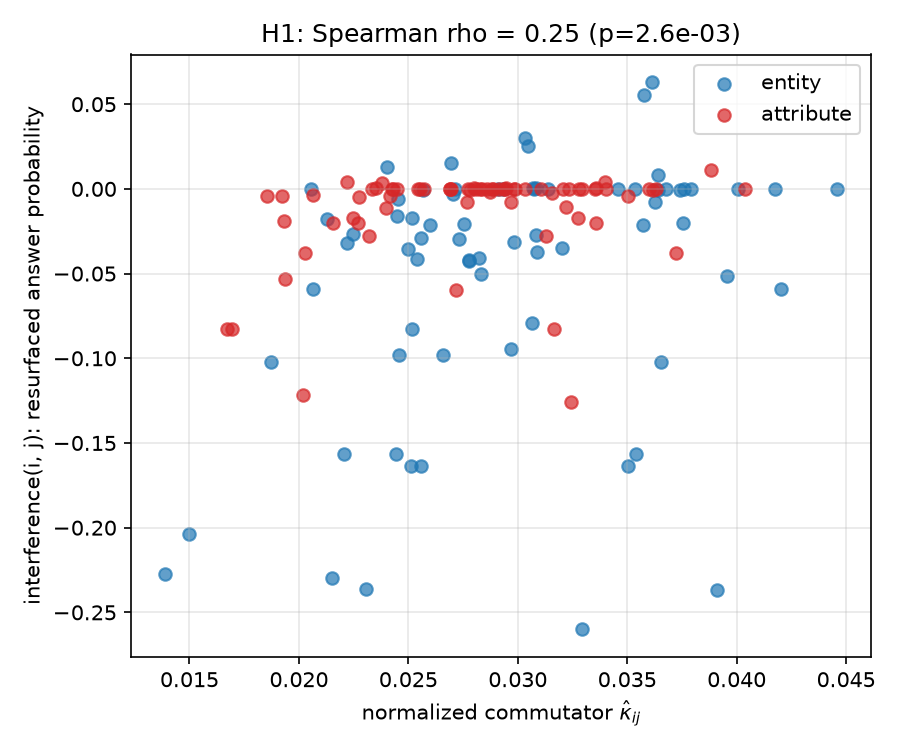
\includegraphics[keepaspectratio,alt={Figure 3. Normalized commutator versus sequential-unlearning interference on Llama-3.2-1B.}]{Exp_H1.png}}
\end{figure}

\textbf{Figure 3. Commutator versus interference (H1, first test).} Each point is a pair of sequential unlearning requests \((i,j)\) on Llama-3.2-1B: the horizontal axis is the normalized commutator \(\hat\kappa_{ij}\), the vertical axis is interference\((i,j)\), the change in request \(i\)'s answer probability caused by a later request \(j\). Blue points are the entity partition, red the attribute partition. Spearman \(\rho=0.25\) (\(p=2.6\times10^{-3}\), \(n=144\)), holding within each condition and, when stratified by pair gap, carried by the multi-step windows (\(\rho=0.40\) at gap 2) with no adjacent-pair signal (\(\rho=-0.02\)); it survives partialling out gap, update magnitude, and condition jointly (\(\rho=0.24\)).

Logging \(\hat\kappa_{ij}\) per adapted layer shows the relationship is distributed rather than localized. The per-layer correlation with interference is positive in fifteen of the sixteen adapters and significant (\(p<0.05\)) in ten, weakest at the earliest adapted layer (layer 8, \(\rho=-0.04\) and \(+0.03\) for its two projections) and strongest at the deep MLP projections of layers 13 and 14 (\(\rho\approx0.33\), \(p\approx7\times10^{-5}\)). The commutator-interference link is therefore a property of the middle-to-late block as a whole rather than any single layer.

Three limits keep this preliminary. The partitions did not separate on \(\hat\kappa\) in the predicted direction (mean \(\hat\kappa\) was \(0.030\) for entity against \(0.028\) for attribute), so the correlation, not the entity-against-attribute contrast, is what carries the result, and the partition as a lever on \(\hat\kappa\) is not supported by this run. The signal is a window statistic, not a pair mechanism: single-step interference between adjacent requests shows no commutator association (\(\rho=-0.02\)), so what the proxy detects is drift accumulated across the window from \(i\) to \(j\), and per-step pair attribution is registered as a secondary metric for the full-harness run rather than claimed here. Forget quality is measured by answer probability on injected facts rather than TOFU's truth-ratio indistinguishability, so the test fixes the direction of H1 but not its magnitude on the benchmark, and the ordering, retain, and utility metrics specified above are not evaluated here. The full-harness version remains the complete test.

\subsection{Matrix-Level BCH Validation}\label{matrix-level-bch-validation}

We first evaluate the second-order BCH approximation in a matrix-only setting, without any neural network, to verify that the implementation behaves as predicted by the Lie group formulation. For each target Frobenius norm

\[
\|A_i\|_F\in\{0.01,0.05,0.1,0.2,0.4,0.8\},
\]

we sample 200 random generator pairs \(A_1,A_2\in\mathfrak{so}(128)\) with \(\|A_1\|_F\approx\|A_2\|_F\approx\texttt{target\_norm}\). For each pair, we compute the exact composition

\[
R_{\mathrm{exact}}=\exp(A_2)\exp(A_1),
\]

and compare it to two approximations:

\[
R_{\mathrm{naive}}=\exp(A_1+A_2),
\qquad
R_{\mathrm{BCH}}=
\exp\left(A_1+A_2+\frac{1}{2}[A_2,A_1]\right).
\]

We measure Frobenius composition error

\[
\Delta_{\mathrm{comp}}=\|R_{\mathrm{exact}}-R_{\mathrm{approx}}\|_F
\]

and also record normalized error \(\Delta_{\mathrm{comp}}/\|R_{\mathrm{exact}}\|_F\), commutator norm \(\|[A_2,A_1]\|_F\), and deviations from skew-symmetry and orthogonality. Table 1 summarizes mean errors over 200 samples per norm level. The improvement column reports the average ratio of naive error to BCH error,

\[
\mathbb{E}\left[
\frac{\Delta_{\mathrm{comp}}^{\mathrm{naive}}}
{\Delta_{\mathrm{comp}}^{\mathrm{BCH}}+\epsilon}
\right].
\]

\textbf{Table 1. Matrix-level BCH composition accuracy.} Mean composition error \(\Delta_{\mathrm{comp}}\) for naive generator addition versus second-order BCH across generator norm regimes. BCH consistently achieves lower error, with 27x-2200x mean improvement over naive addition.

{\def\LTcaptype{none} % do not increment counter
\begin{longtable}[]{@{}llll@{}}
\toprule\noalign{}
target\_norm & naive\_mean & bch\_mean & improvement\_mean \\
\midrule\noalign{}
\endhead
\bottomrule\noalign{}
\endlastfoot
0.01 & 6.0e-06 & 2.9e-09 & 2.2e3 \\
0.05 & 1.6e-04 & 3.6e-07 & 4.3e2 \\
0.10 & 6.2e-04 & 2.9e-06 & 2.2e2 \\
0.20 & 2.5e-03 & 2.3e-05 & 1.1e2 \\
0.40 & 9.9e-03 & 1.8e-04 & 5.4e1 \\
0.80 & 4.0e-02 & 1.5e-03 & 2.7e1 \\
\end{longtable}
}

\begin{figure}
\centering
\pandocbounded{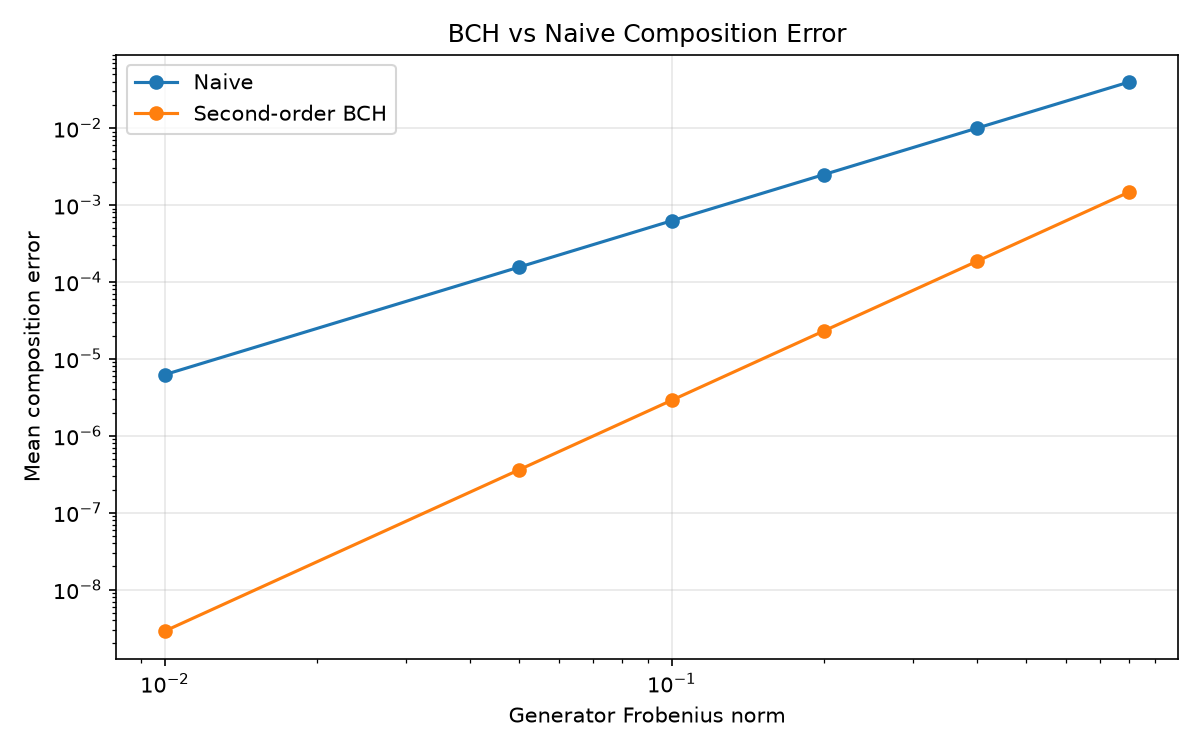
\includegraphics[keepaspectratio,alt={Figure 1(a). BCH vs Naive Composition Error.}]{Exp1_1.png}}
\end{figure}

\begin{figure}
\centering
\pandocbounded{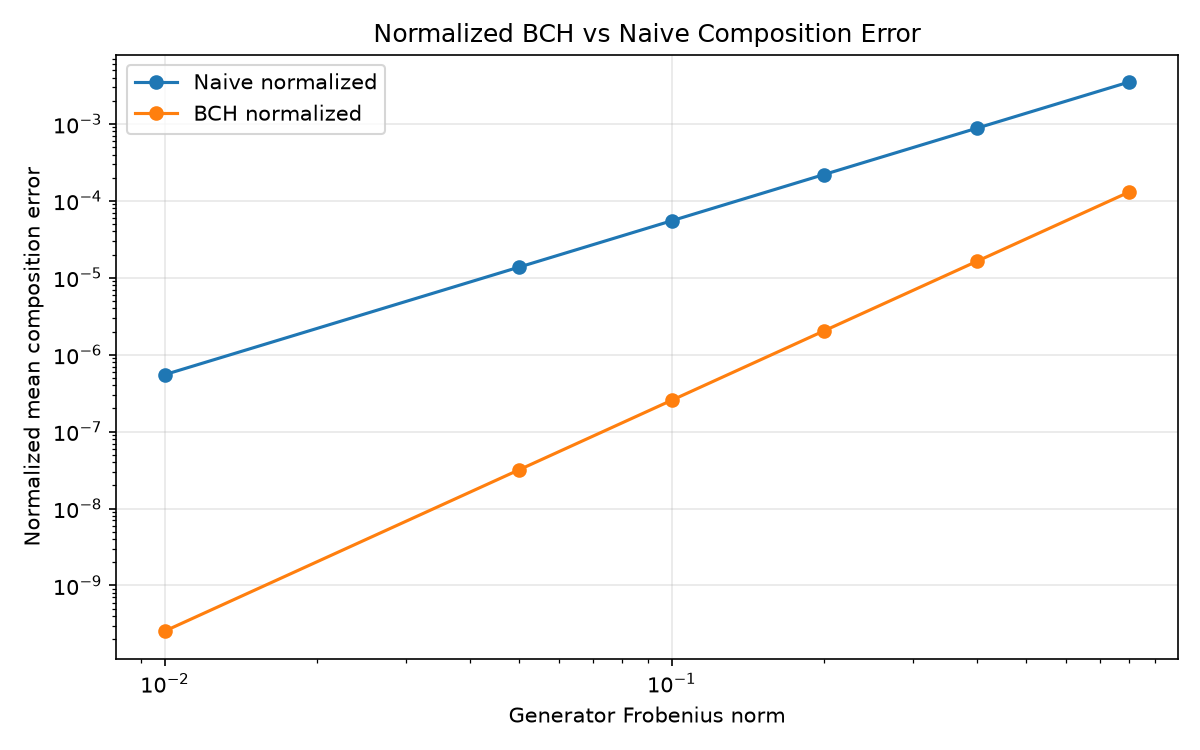
\includegraphics[keepaspectratio,alt={Figure 1(b). Normalized BCH vs Naive Composition Error.}]{Exp1_2.png}}
\end{figure}

\begin{figure}
\centering
\pandocbounded{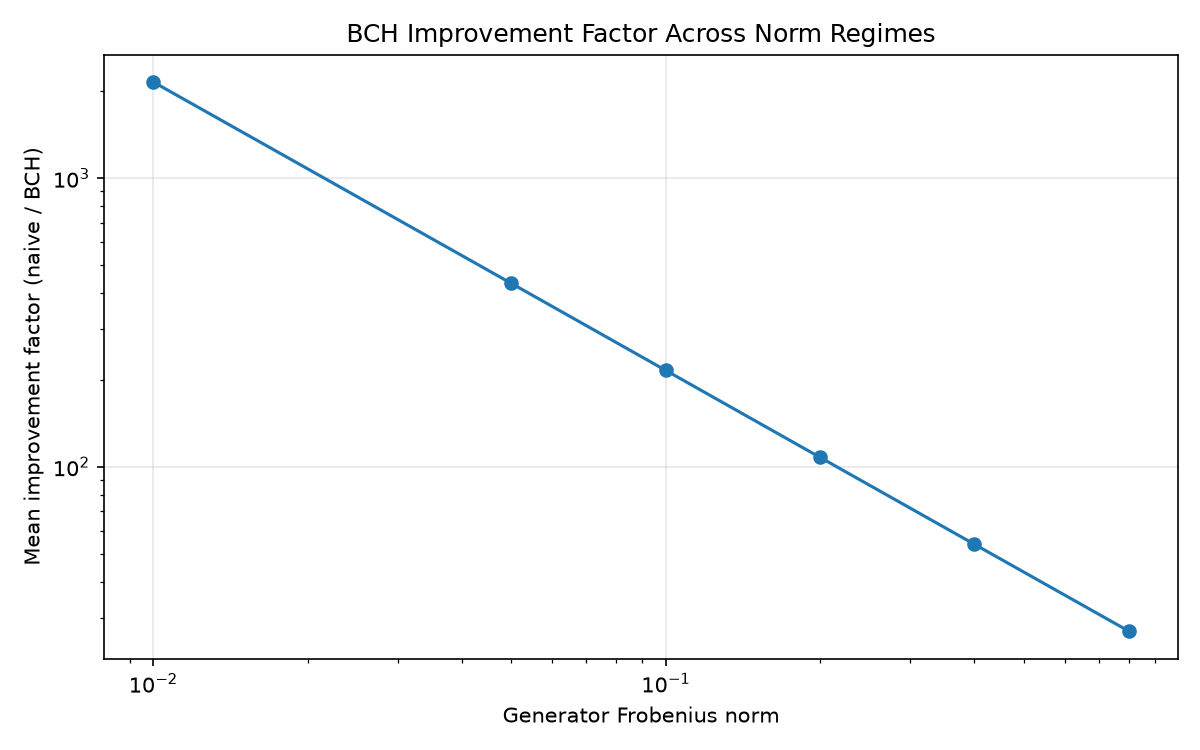
\includegraphics[keepaspectratio,alt={Figure 1(c). BCH Improvement Factor Across Norm Regimes.}]{Exp1_3.png}}
\end{figure}

\textbf{Figure 1. Matrix-level BCH validation.} (a) BCH vs Naive Composition Error. (b) Normalized BCH vs Naive Composition Error. (c) BCH Improvement Factor Across Norm Regimes.

Figure 1(a) plots the mean absolute composition error as a function of generator Frobenius norm for both approximations. The naive error increases rapidly with the norm of the generators, while the BCH error remains substantially lower in every regime we consider. In the smallest-norm setting, \(\|A_i\|_F\approx 0.01\), the BCH approximation reduces mean composition error by roughly three orders of magnitude relative to naive addition. Even at the largest norm tested, \(\|A_i\|_F\approx 0.8\), BCH still improves mean error by a factor of about 27x.

Figure 1(b) shows the same comparison after normalizing by \(\|R_{\mathrm{exact}}\|_F\). The normalized curves exhibit the same pattern: second-order BCH tracks the exact composition more closely than naive generator addition at all norms studied. Figure 1(c) reports the mean improvement factor \(\mathbb{E}[\Delta_{\mathrm{comp}}^{\mathrm{naive}}/\Delta_{\mathrm{comp}}^{\mathrm{BCH}}]\) as a function of generator norm, which decays smoothly from approximately \(2.2\times 10^3\) at \(\|A_i\|_F=0.01\) to approximately \(27\) at \(\|A_i\|_F=0.8\). This behavior is consistent with the theoretical small-angle regime: BCH offers the largest gains when \(\|A\|\) is small, but remains beneficial even for moderate norms.

Across all configurations, deviations from skew-symmetry and orthogonality remain at machine precision. The average skew-symmetry violation of the BCH generator,

\[
\|A_{\mathrm{BCH}}+A_{\mathrm{BCH}}^\top\|_F,
\]

is on the order of \(10^{-14}\), and the average orthogonality error

\[
\|\exp(A_{\mathrm{BCH}})^\top\exp(A_{\mathrm{BCH}})-I\|_F
\]

is similarly negligible. These results confirm that the numerical implementation respects the Lie algebra and Lie group structure to within floating-point error, and they support the use of second-order BCH-aware accumulation as a more accurate model of sequential orthogonal updates than naive generator addition in this matrix-level setting.

We further test the rank-truncation term of Theorem 1 by extending this study: at fixed generator norm we sweep the truncation rank \(R\) and compare the measured composition error of rank-truncated BCH accumulation against the two-term bound, evaluated in its small-angle (\(L=1\)) form with the running-\(\rho\) BCH remainder \(\sum_t\beta_t\) and the measured Eckart-Young tails \(\sum_t\tau_t\). The generators have per-task rank \(2r=8\) in \(\mathfrak{so}(128)\); we sweep \(\varepsilon\in[0.01,0.4]\), \(T\in\{8,16\}\), and \(R\in\{r,2r,4r,\infty\}\).

Theorem 1 governs the runs whose accumulated history stays inside its radius, \(\max_t(\varepsilon+\|H_t\|_F)<\ln 2\); in this ensemble that holds up to \(\varepsilon\approx 0.18\) at \(T=8\) and \(\varepsilon\approx 0.14\) at \(T=16\) (marked in Figure 1(d)). Inside the regime the bound holds as guaranteed. At \(\varepsilon=0.10\), \(T=8\), where \(\max_t(\varepsilon+\|H_t\|_F)=0.38\), the Eckart-Young term shrinks from \(0.61\) at \(R=r\) to \(0.21\) at \(R=4r\), reaching machine precision once \(2R\) covers the occupied rank, and the realized error follows it (\(0.23\), \(0.18\), \(0.11\) against the bound's \(0.61\), \(0.46\), \(0.23\)); the two error sources of Theorem 1 are separately visible and jointly bounded. Beyond the marked crossing the hypothesis fails and \(L=(2-e^{\varepsilon+\rho})^{-1}\) is undefined, so the plotted small-angle expression is no longer a guarantee; we report it there only as an empirical envelope, and it continued to dominate the realized error for this ensemble at every point tested (for instance \(1.39\) against the envelope's \(6.7\) at the \(\varepsilon=0.4\), \(T=16\) corner). Throughout, the truncated accumulation stays skew-symmetric and orthogonal to \(10^{-15}\).

\begin{figure}
\centering
\pandocbounded{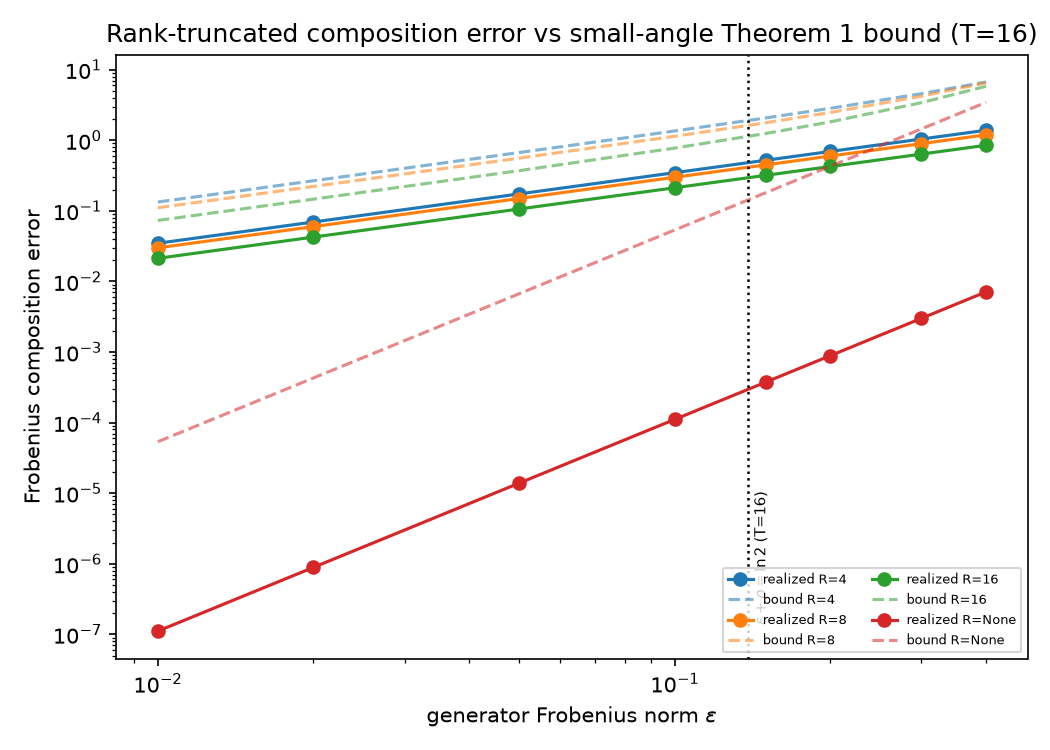
\includegraphics[keepaspectratio,alt={Figure 1(d). Rank-truncated composition error versus the Theorem 1 bound.}]{Exp1_4.png}}
\end{figure}

\textbf{Figure 1(d).} Measured composition error of rank-truncated BCH accumulation (solid) against the two-term Theorem 1 bound in its small-angle \(L=1\) form (dashed; running-\(\rho\) BCH remainder plus measured Eckart-Young tail), versus generator Frobenius norm and truncation rank \(R\) in \(\mathfrak{so}(128)\) at \(T=16\). The dotted vertical line marks where the accumulated history leaves Theorem 1's radius, \(\varepsilon+\rho=\ln 2\) (\(\varepsilon\approx 0.14\) at \(T=16\)): left of it the bound is guaranteed, right of it it is reported as an empirical envelope.

\subsection{Toy MLP Geometry and Retain-Constraint}\label{toy-mlp-geometry-and-retain-constraint}

To test the proposed geometry and retain-constraint mechanisms in a controlled trained-network setting, we construct a two-layer MLP on MNIST. The model has a single hidden layer with 256 units and no bias in the first linear layer, which defines a pretrained weight matrix \(W\in\mathbb{R}^{256\times 784}\). After training on a balanced subset of MNIST to 97\% accuracy, we freeze all parameters and apply adaptation only through this layer. The forget set \(\mathcal{D}_f\) consists of images from a single digit class, digit 7, while the retain set \(\mathcal{D}_r\) contains images from all remaining classes.

\paragraph{Geometry preservation at the weight level}\label{geometry-preservation-at-the-weight-level}

We first compare geometry preservation across three update parameterizations applied to \(W\): additive low-rank updates in a LoRA-style form, first-order skew updates of the form \(W'=(I+A)W\), and exact exponential skew updates \(W'=\exp(A)W\) with \(A\in\mathfrak{so}(256)\). For each target generator norm

\[
\|A\|_F\in\{0.01,0.05,0.1,0.2,0.4\},
\]

we sample 20 random skew generators, construct corresponding updates with matched effective update norms, and measure normalized Gram deviation

\[
\overline{\Delta}_G=
\frac{\|W^\top W-W'^\top W'\|_F}{\|W^\top W\|_F}.
\]

\begin{figure}
\centering
\pandocbounded{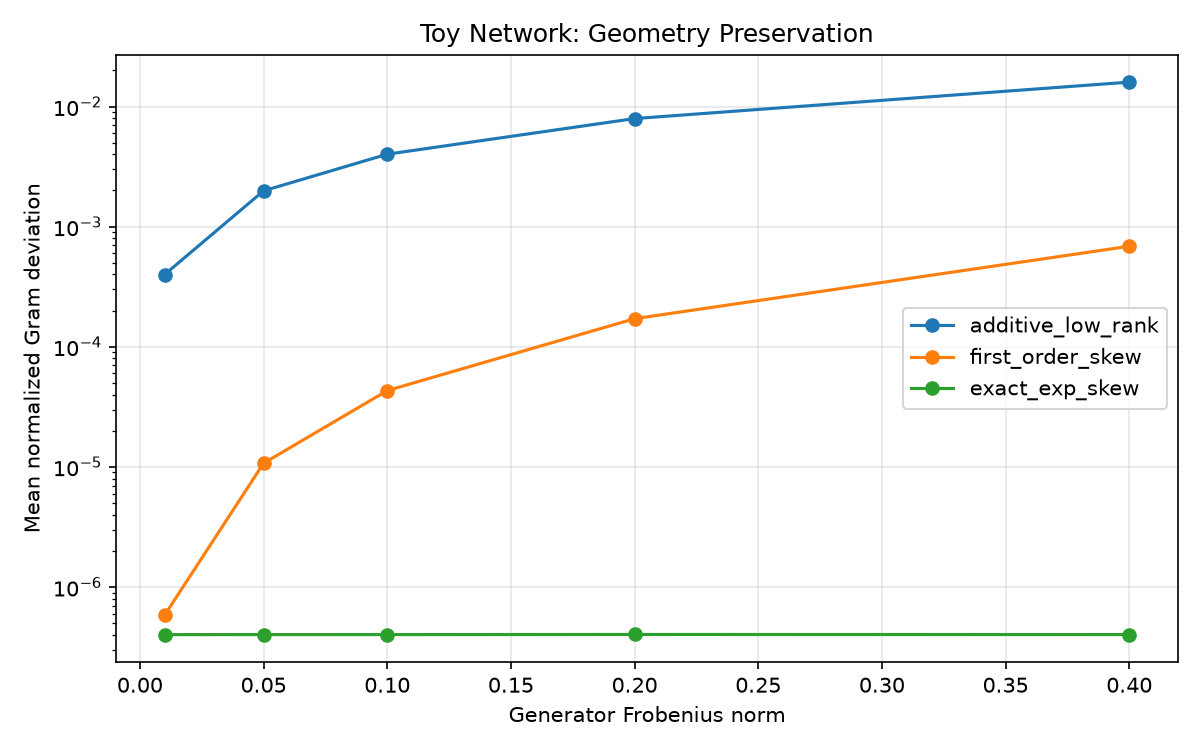
\includegraphics[keepaspectratio,alt={Figure 2(a). Toy network geometry preservation.}]{Exp2_1.png}}
\end{figure}

\textbf{Figure 2(a). Toy network geometry preservation.} Mean normalized Gram deviation \(\overline{\Delta}_G\) for additive low-rank, first-order skew, and exact exponential skew updates applied to the first-layer weight matrix of a pretrained MNIST MLP, as a function of generator Frobenius norm.

Figure 2(a) reports the mean normalized Gram deviation as a function of generator norm for the three methods. Additive low-rank updates show increasing Gram distortion, from \(\overline{\Delta}_G\approx 4.0\times 10^{-4}\) at \(\|A\|_F=0.01\) to \(\overline{\Delta}_G\approx 1.6\times 10^{-2}\) at \(\|A\|_F=0.4\). First-order skew updates exhibit smaller but still growing distortion, reaching \(\overline{\Delta}_G\approx 6.9\times 10^{-4}\) at the largest norm. In contrast, exponential skew updates maintain \(\overline{\Delta}_G\approx 4.0\times 10^{-7}\) across all norms, effectively at numerical precision and orders of magnitude lower than the additive and first-order baselines. These results empirically confirm that the exponential parameterization preserves the Gram geometry of the adapted weight matrix in this toy network, while approximate rotational and additive parameterizations do not, even under matched update magnitudes.

\paragraph{Retain-gradient projection and forget-retain trade-off}\label{retain-gradient-projection-and-forget-retain-trade-off}

We next study the retain-gradient projection in a toy unlearning setup. The forget objective encourages the model to map all forget-class examples to a fixed scrambled target label, while the retain objective is the standard cross-entropy on the retain set. We compare four adapters on the frozen MLP: an additive low-rank adapter in a LoRA-style form, a first-order skew adapter, an exponential skew adapter without retain projection, and an exponential skew adapter with retain-gradient projection. The retain subspace is estimated by collecting retain gradients for \(W\) on minibatches from \(\mathcal{D}_r\), constructing the corresponding retain generators \(S_r\), and extracting a low-dimensional basis \(U_k\) that captures approximately 95\% of the energy of the stacked retain generators.

Each adapter is trained on \(\mathcal{D}_f\) until the forget loss on the forget-class test split reaches a small common target, and is then evaluated on both forget and retain test splits. At the end of training, we measure the change in retain loss,

\[
\Delta_{\mathrm{retain}}=L_r(W')-L_r(W),
\]

the change in retain accuracy, the normalized Gram deviation \(\overline{\Delta}_G\), and the alignment of the final generator with the estimated retain subspace.

\begin{figure}
\centering
\pandocbounded{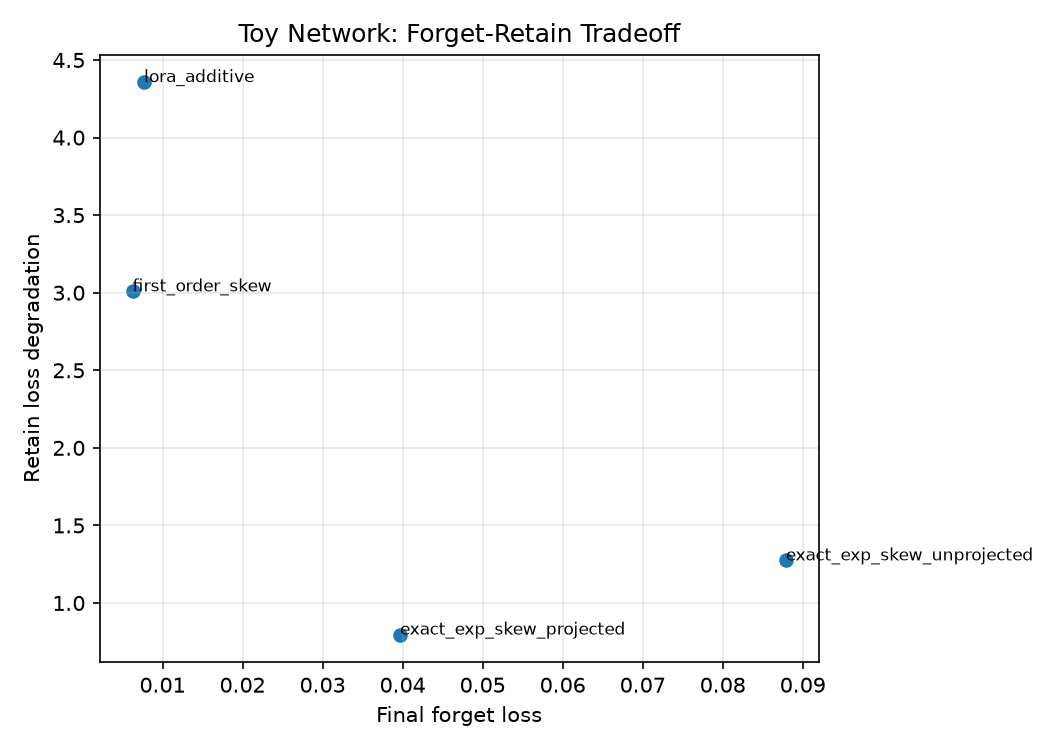
\includegraphics[keepaspectratio,alt={Figure 2(b). Toy MLP forget-retain trade-off.}]{Exp2_2.png}}
\end{figure}

\textbf{Figure 2(b). Toy MLP forget-retain trade-off.} Retain loss degradation versus final forget loss for additive low-rank, first-order skew, exponential skew, and retain-projected exponential skew adapters on the frozen MNIST MLP.

Figure 2(b) plots retain loss degradation versus final forget loss for the four methods. The additive low-rank and first-order skew baselines achieve very low forget loss but incur the largest retain damage, with retain loss increases of roughly 4.4 and 3.1 respectively on the retain test set, accompanied by substantial Gram distortion of the adapted weight. Exponential skew updates yield much smaller retain degradation. The unprojected exponential adapter increases retain loss by about 1.32, while the retain-projected exponential adapter further reduces retain loss degradation to about 1.10, at the operating points each method reached (forget loss 0.04 projected, 0.088 unprojected; the additive baselines reach 0.007). The projected exponential adapter also exhibits lower alignment with the estimated retain subspace, approximately 0.11 versus 0.36 for the unprojected exponential adapter, consistent with the intended constraint that the update generator remains orthogonal to retain-gradient directions.

These toy experiments provide an interpretable sanity check. Exponential skew updates preserve the Gram geometry of the adapted weight in a trained network, and retain-gradient projection reduces collateral damage on retained data in this setting, though the methods stop at different forget-loss levels. The transformer experiments of Section 6.2 therefore compare full training trajectories, so that matched-forget comparisons are read off curves rather than endpoints.

\subsection{Ablations}\label{ablations}

The minimum ablation package:

\begin{enumerate}
\def\labelenumi{\arabic{enumi}.}
\tightlist
\item
  Removing retain-gradient projection (tests Proposition 2 at scale).
\item
  Removing BCH correction, i.e., naive generator addition (tests H2).
\item
  Removing commutator regularization (\(\lambda_{\mathrm{BCH}}=0\)).
\item
  Per-task rank \(r\) sweep (capacity).
\item
  Truncation rank \(R\in\{r,2r,4r,\text{full}\}\) (tests the Eckart-Young term \(\tau_t\) of Theorem 1).
\item
  Retain-basis refresh period \(k\) and energy fraction \(\rho_E\) (the staleness and coverage trade-off of Section 3.4).
\item
  Norm bound \(\varepsilon\) and history bound \(\rho_{\max}\), with clip-activation \(\kappa_t\) logged (the regime of the Remark after Theorem 1).
\end{enumerate}

Each ablation is reported against the claim it tests: rank against capacity, truncation rank against the Eckart-Young term, refresh parameters against the failure modes of Section 3.4, and norm bounds against the theorem's regime of validity.

\section{Interpretation and Limitations}\label{interpretation-and-limitations}

\subsection{Continual learning as non-commutative motion}\label{continual-learning-as-non-commutative-motion}

Additive frameworks treat task order as irrelevant, because \(\Delta_1+\Delta_2=\Delta_2+\Delta_1\). Multiplicative orthogonal updates do not, and their order dependence is carried by the commutators, which appear as explicit second-order terms in the accumulated generator. The reading this suggests is that continual adaptation should control not only how large each update is but how compatible it is with the ones already applied, measured through commutator structure. The commutator regularizer of Section 3.9 and the composition bound of Theorem 1 are two ways to act on that structure.

\subsection{Capacity as Lie algebra allocation}\label{capacity-as-lie-algebra-allocation}

The full algebra \(\mathfrak{so}(n)\) has \(n(n-1)/2\) dimensions, but scalable implementations use a low-rank or otherwise structured subset. Continual adaptation is then the allocation of a limited budget of rotational directions across tasks, and interference is expected to grow when tasks demand incompatible, non-commuting directions. This gives a geometric account of capacity in which interference depends not only on parameter count but on how update directions interact algebraically, and it is what the truncation-rank budget \(R\) of Theorem 1 trades against fidelity.

\subsection{Limitations}\label{limitations}

The one exact guarantee is parameter-space. Applying \(\exp(A)W\) with \(A\in\mathfrak{so}(n)\) preserves the column Gram matrix \(W^\top W\), and with it column norms, inner products, and angles, independently of the data and without any small-angle approximation. It does not follow that the network's function is preserved: transformer behavior depends on nonlinear activations, normalization, residual paths, and composition with many other matrices, so \(f(x;W)\neq f(x;\exp(A)W)\) in general. The geometry controls one source of drift, not the semantics, and whether parameter-space preservation predicts behavioral retention is the open question the invariant-validity analysis is meant to settle. It may settle it negatively.

Three further limits bound the claims. The retain constraint is first-order and local: it controls infinitesimal retain-loss variation, not global retention after finite updates or after nonlinear propagation. The composition analysis truncates BCH at second order and holds the history at fixed rank; Theorem 1 bounds the resulting error under a norm condition, but long sequences with large nested commutators fall outside that regime. And the low-rank generator restricts the accessible rotation directions, so a target change lying outside the low-rank subspace can leave the forget objective underfit.

These limits set the agenda. The parameter-space invariants studied here should be connected to representation- and output-space metrics in transformers; the exponential and Cayley parameterizations should be compared under identical budgets; and commutator-aware scheduling, ordering tasks to reduce interference before optimization begins, is worth testing once the interference-commutator link is measured.

\section{Conclusion}\label{conclusion}

This paper recast sequential adaptation and targeted unlearning as non-commutative composition of orthogonal updates: each edit is a rotation \(\exp(A)W\) generated by a skew-symmetric \(A\), a sequence is a product of exponentials, and interference between edits is carried by the commutators \([A_i, A_j]\). Three contributions follow. Theorem 1 bounds the error of rank-truncated second-order BCH accumulation, separating a norm-controlled BCH term from an Eckart-Young truncation tail. The method is an exact low-rank exponential adapter, differentiated through the matrix exponential, with retain-gradient projection carried out in \(\mathfrak{so}(n)\) and fixed-rank composition, at LoRA-order cost. And the evaluation treats the link from parameter-space geometry to behavioral retention as a hypothesis with a specified test, not an assumption.

The established evidence is deliberately scoped: geometry preservation and second-order composition accuracy are confirmed at the matrix level and in a small trained network. Of the two claims that matter in practice, one now has direct evidence and one is still open. A first test on Llama-3.2-1B supports the interference claim, with commutator magnitude predicting pairwise sequential interference (Spearman \(\rho=0.25\), holding within conditions and after controlling for update magnitude); what remains for it is the scale of the effect under the full benchmark harness. The retention claim, that retain projection reduces collateral damage at matched forget performance in transformers, is still stated so that it can fail, and the experiments of Section 6 are designed to let it. Whatever the outcome, the framework's purpose is to make continual adaptation inspectable: update magnitude, retention pressure, and order dependence are explicit mathematical objects to be measured rather than assumed.

\section{Reproducibility}\label{reproducibility}

All experiments are produced by a single configuration-driven pipeline, and every figure regenerates from raw logs with one command (\texttt{python\ make\_figures.py}). Code, configurations, seeds, and CSV logs are archived at https://doi.org/10.5281/zenodo.21267659 and mirrored at https://github.com/design-smith/lie-algebraic-unlearning-release.

\section{References}\label{references}

Absil, P.-A., Mahony, R., \& Sepulchre, R. (2008). \emph{Optimization Algorithms on Matrix Manifolds}. Princeton University Press.

Arjovsky, M., Shah, A., \& Bengio, Y. (2016). Unitary Evolution Recurrent Neural Networks. \emph{International Conference on Machine Learning}. arXiv:1511.06464.

Bourtoule, L., Chandrasekaran, V., Choquette-Choo, C. A., Jia, H., Travers, A., Zhang, B., Lie, D., \& Papernot, N. (2021). Machine Unlearning. \emph{IEEE Symposium on Security and Privacy}. arXiv:1912.03817.

Chaudhry, A., Ranzato, M., Rohrbach, M., \& Elhoseiny, M. (2019). Efficient Lifelong Learning with A-GEM. \emph{International Conference on Learning Representations}. arXiv:1812.00420.

Dettmers, T., Pagnoni, A., Holtzman, A., \& Zettlemoyer, L. (2023). QLoRA: Efficient Finetuning of Quantized LLMs. \emph{Advances in Neural Information Processing Systems}. arXiv:2305.14314.

Dorna, V., et al.~(2025). OpenUnlearning: Accelerating LLM Unlearning via Unified Benchmarking of Methods and Metrics. \emph{Advances in Neural Information Processing Systems, Datasets and Benchmarks Track}. arXiv:2506.12618.

Eldan, R., \& Russinovich, M. (2023). Who's Harry Potter? Approximate Unlearning in LLMs. arXiv:2310.02238.

Farajtabar, M., Azizan, N., Mott, A., \& Li, A. (2020). Orthogonal Gradient Descent for Continual Learning. \emph{Artificial Intelligence and Statistics (AISTATS)}. arXiv:1910.07104.

Gallier, J., \& Quaintance, J. (2020). \emph{Differential Geometry and Lie Groups: A Computational Perspective}. Springer.

Gao, C., Wang, L., Weng, C., Wang, X., \& Zhu, Q. (2024). Practical Unlearning for Large Language Models. arXiv:2407.10223.

Hall, B. C. (2015). \emph{Lie Groups, Lie Algebras, and Representations: An Elementary Introduction} (2nd ed.). Springer.

Helfrich, K., Willmott, D., \& Ye, Q. (2018). Orthogonal Recurrent Neural Networks with Scaled Cayley Transform. \emph{International Conference on Machine Learning}. arXiv:1707.09520.

Higham, N. J. (2008). \emph{Functions of Matrices: Theory and Computation}. Society for Industrial and Applied Mathematics.

Houlsby, N., Giurgiu, A., Jastrzebski, S., Morrone, B., de Laroussilhe, Q., Gesmundo, A., Attariyan, M., \& Gelly, S. (2019). Parameter-Efficient Transfer Learning for NLP. \emph{International Conference on Machine Learning}. arXiv:1902.00751.

Hu, E. J., Shen, Y., Wallis, P., Allen-Zhu, Z., Li, Y., Wang, S., Wang, L., \& Chen, W. (2022). LoRA: Low-Rank Adaptation of Large Language Models. \emph{International Conference on Learning Representations}. arXiv:2106.09685.

Hu, J., Huang, Z., Yin, X., Ruan, W., Cheng, G., Dong, Y., \& Huang, X. (2025). FALCON: Fine-grained Activation Manipulation by Contrastive Orthogonal Unalignment for Large Language Models. arXiv:2502.01472.

Ilharco, G., Ribeiro, M. T., Wortsman, M., Gururangan, S., Schmidt, L., Hajishirzi, H., \& Farhadi, A. (2023). Editing Models with Task Arithmetic. \emph{International Conference on Learning Representations}. arXiv:2212.04089.

Jang, J., Yoon, D., Yang, S., Cha, S., Lee, M., Logeswaran, L., \& Seo, M. (2023). Knowledge Unlearning for Mitigating Privacy Risks in Language Models. \emph{Association for Computational Linguistics}. arXiv:2210.01504.

Kirkpatrick, J., Pascanu, R., Rabinowitz, N., Veness, J., Desjardins, G., Rusu, A. A., et al.~(2017). Overcoming Catastrophic Forgetting in Neural Networks. \emph{Proceedings of the National Academy of Sciences}, 114(13), 3521-3526. arXiv:1612.00796.

Lester, B., Al-Rfou, R., \& Constant, N. (2021). The Power of Scale for Parameter-Efficient Prompt Tuning. \emph{Empirical Methods in Natural Language Processing}. arXiv:2104.08691.

Lezcano-Casado, M. (2019). Trivializations for Gradient-Based Optimization on Manifolds. \emph{Advances in Neural Information Processing Systems}. arXiv:1909.09501.

Lezcano-Casado, M., \& Martinez-Rubio, D. (2019). Cheap Orthogonal Constraints in Neural Networks: A Simple Parametrization of the Orthogonal and Unitary Group. \emph{International Conference on Machine Learning}. arXiv:1901.08428.

Li, N., Pan, A., Gopal, A., Yue, S., Berrios, D., Gatti, A., \ldots{} Hendrycks, D. (2024). The WMDP Benchmark: Measuring and Reducing Malicious Use with Unlearning. \emph{International Conference on Machine Learning}. arXiv:2403.03218.

Li, X. L., \& Liang, P. (2021). Prefix-Tuning: Optimizing Continuous Prompts for Generation. \emph{Association for Computational Linguistics}. arXiv:2101.00190.

Liu, S., Yao, Y., Jia, J., Casper, S., Baracaldo, N., Hase, P., Yao, Y., Liu, C. Y., Xu, X., Li, H., Varshney, K. R., Bansal, M., Koyejo, S., \& Liu, Y. (2024). Rethinking Machine Unlearning for Large Language Models. arXiv:2402.08787.

Liu, S.-Y., Wang, C.-Y., Yin, H., Molchanov, P., Wang, Y.-C. F., Cheng, K.-T., \& Chen, M.-H. (2024). DoRA: Weight-Decomposed Low-Rank Adaptation. \emph{International Conference on Machine Learning}. arXiv:2402.09353.

Liu, W., Qiu, Z., Feng, Y., Xiu, Y., Xue, Y., Yu, L., Feng, H., Liu, Z., Heo, J., Peng, S., Wen, Y., Black, M. J., Weller, A., \& Schoelkopf, B. (2024). Parameter-Efficient Orthogonal Finetuning via Butterfly Factorization. \emph{International Conference on Learning Representations}. arXiv:2311.06243.

Lopez-Paz, D., \& Ranzato, M. (2017). Gradient Episodic Memory for Continual Learning. \emph{Advances in Neural Information Processing Systems}. arXiv:1706.08840.

Lynch, A., Guo, P., Ewart, A., Casper, S., \& Hadfield-Menell, D. (2024). Eight Methods to Evaluate Robust Unlearning in LLMs. arXiv:2402.16835.

Maini, P., Feng, Z., Schwarzschild, A., Lipton, Z. C., \& Kolter, J. Z. (2024). TOFU: A Task of Fictitious Unlearning for LLMs. \emph{Conference on Language Modeling (COLM)}. arXiv:2401.06121.

Mhammedi, Z., Hellicar, A., Rahman, A., \& Bailey, J. (2017). Efficient Orthogonal Parametrisation of Recurrent Neural Networks Using Householder Reflections. \emph{International Conference on Machine Learning}. arXiv:1612.00188.

Qiu, Z., Liu, W., Feng, H., Xue, Y., Feng, Y., Liu, Z., Zhang, D., Weller, A., \& Schoelkopf, B. (2023). Controlling Text-to-Image Diffusion by Orthogonal Finetuning. \emph{Advances in Neural Information Processing Systems}. arXiv:2306.07280.

Rossmann, W. (2002). \emph{Lie Groups: An Introduction Through Linear Groups}. Oxford University Press.

Saha, G., Garg, I., \& Roy, K. (2021). Gradient Projection Memory for Continual Learning. \emph{International Conference on Learning Representations}. arXiv:2103.09762.

Shi, W., Lee, J., Huang, Y., Malladi, S., Zhao, J., Holtzman, A., Liu, D., Zettlemoyer, L., Smith, N. A., \& Zhang, C. (2024). MUSE: Machine Unlearning Six-Way Evaluation for Language Models. arXiv:2407.06460.

Van Loan, C. F. (1978). Computing Integrals Involving the Matrix Exponential. \emph{IEEE Transactions on Automatic Control}, 23(3), 395-404.

Wang, S., Li, X., Sun, J., \& Xu, Z. (2021). Training Networks in Null Space of Feature Covariance for Continual Learning. \emph{Conference on Computer Vision and Pattern Recognition}. arXiv:2103.07113.

Wortsman, M., Ilharco, G., Gadre, S. Y., Roelofs, R., Gontijo-Lopes, R., Morcos, A. S., et al.~(2022). Model Soups: Averaging Weights of Multiple Fine-tuned Models Improves Accuracy Without Increasing Inference Time. \emph{International Conference on Machine Learning}. arXiv:2203.05482.

Yadav, P., Tam, D., Choshen, L., Raffel, C., \& Bansal, M. (2023). TIES-Merging: Resolving Interference When Merging Models. \emph{Advances in Neural Information Processing Systems}. arXiv:2306.01708.

Yuan, S., Liu, H., \& Xu, H. (2024). Bridging the Gap between Low-rank and Orthogonal Adaptation via Householder Reflection Adaptation. \emph{Advances in Neural Information Processing Systems}. arXiv:2405.17484.

Yao, J., Chien, E., Du, M., Niu, X., Wang, T., Cheng, Z., \& Yue, X. (2024). Machine Unlearning of Pre-trained Large Language Models. \emph{Association for Computational Linguistics}. arXiv:2402.15159.

Zhang, R., Lin, L., Bai, Y., \& Mei, S. (2024). Negative Preference Optimization: From Catastrophic Collapse to Effective Unlearning. arXiv:2404.05868.

\section{Appendix A. Additional Derivations}\label{appendix-a.-additional-derivations}

\subsection{\texorpdfstring{A.1 Projection onto \(\mathfrak{so}(n)\)}{A.1 Projection onto \textbackslash mathfrak\{so\}(n)}}\label{a.1-projection-onto-mathfrakson}

Every square matrix \(M\in\mathbb{R}^{n\times n}\) decomposes into symmetric and skew-symmetric parts:

\[
M=\frac{1}{2}(M+M^\top)+\frac{1}{2}(M-M^\top).
\]

The two components are orthogonal under the Frobenius inner product. Therefore the orthogonal projection of \(M\) onto \(\mathfrak{so}(n)\) is

\[
P_{\mathfrak{so}}(M)=\frac{1}{2}(M-M^\top).
\]

\subsection{A.2 Exact gradient of the exponential objective}\label{a.2-exact-gradient-of-the-exponential-objective}

The exact gradient of \(J(A)=L_f(\exp(A)W)\) used by the method is derived in Appendix B, together with its block-matrix evaluation. The small-generator form \(g_A=\tfrac{1}{2}(G_fW^\top-WG_f^\top)\) is only its \(\|A\|\to 0\) limit and is not used by the method.

\subsection{A.3 Gradient of the Commutator Penalty}\label{a.3-gradient-of-the-commutator-penalty}

Let

\[
C=[A,A_{\mathrm{hist}}]=AA_{\mathrm{hist}}-A_{\mathrm{hist}}A
\]

and

\[
L_{\mathrm{BCH}}=\|C\|_F^2.
\]

The differential is

\[
dC=dA\,A_{\mathrm{hist}}-A_{\mathrm{hist}}\,dA.
\]

Therefore

\[
dL_{\mathrm{BCH}}
=2\langle C,dC\rangle_F
=2\langle C,dA\,A_{\mathrm{hist}}-A_{\mathrm{hist}}dA\rangle_F.
\]

Rearranging traces gives

\[
\nabla_A L_{\mathrm{BCH}}
=2(CA_{\mathrm{hist}}^\top-A_{\mathrm{hist}}^\top C).
\]

Since \(A_{\mathrm{hist}}^\top=-A_{\mathrm{hist}}\),

\[
\nabla_A L_{\mathrm{BCH}}
=2(A_{\mathrm{hist}}C-CA_{\mathrm{hist}}).
\]

\section{Appendix B. Proof of Theorem 1 with Explicit Constants}\label{appendix-b.-proof-of-theorem-1-with-explicit-constants}

Throughout, \(\|\cdot\|_F\) is the Frobenius norm, \(\|\cdot\|_2\) the operator norm, and \(\varepsilon+\rho<\ln 2\). Recall the setup of Theorem 1: per-task generators \(A_1,\dots,A_T\in\mathfrak{so}(n)\) with \(\|A_t\|_F\leq\varepsilon\); the exact accumulation \(H_t=\Phi_{A_t}(H_{t-1})\) with \(\Phi_A(X)=\log(\exp(A)\exp(X))\) and \(H_0=0\); and the truncated-clipped accumulation \(\hat{B}_t=\tilde{H}_{t-1}+A_t+\tfrac{1}{2}[A_t,\tilde{H}_{t-1}]\), \(\breve{B}_t=\mathcal{T}_{2R}(\hat{B}_t)\), \(\tilde{H}_t=\Pi_{\rho_{\max}}(\breve{B}_t)\). The hypothesis gives \(\|H_t\|_F,\|\tilde{H}_t\|_F\leq\rho\).

\subsection{B.0 Exact gradient of the exponential objective}\label{b.0-exact-gradient-of-the-exponential-objective}

For \(J(A)=L_f(\exp(A)W)\) with \(G_f=\nabla_{W_{\mathrm{new}}}L_f\), the Fréchet derivative of the exponential is \(D\exp_A[V]=\int_0^1\exp((1-\tau)A)V\exp(\tau A)\,d\tau\), so the directional derivative is \(DJ(A)[V]=\langle G_f,D\exp_A[V]\,W\rangle_F=\langle G_fW^\top,D\exp_A[V]\rangle_F\). Taking the adjoint of \(D\exp_A\) under the Frobenius inner product, the cyclic-trace identity gives \(\langle D\exp_A[V],X\rangle_F=\langle V,D\exp_{A^\top}[X]\rangle_F\), so the ambient gradient is

\[
\nabla_A J=D\exp_{A^\top}[G_fW^\top].
\]

It is evaluated exactly as the top-right \(n\times n\) block of a \(2n\times 2n\) exponential,

\[
\exp\begin{pmatrix}A^\top & G_fW^\top\\ 0 & A^\top\end{pmatrix}
=\begin{pmatrix}\exp(A^\top) & D\exp_{A^\top}[G_fW^\top]\\ 0 & \exp(A^\top)\end{pmatrix},
\]

a standard identity for the Fréchet derivative of the matrix exponential (Van Loan, 1978; Higham, 2008), or equivalently by reverse-mode differentiation through \(\exp\). The Lie-algebra gradient is \(g_A=P_{\mathfrak{so}}(\nabla_A J)=\tfrac{1}{2}(\nabla_A J-(\nabla_A J)^\top)\). The form \(g_A=\tfrac{1}{2}(G_fW^\top-WG_f^\top)\) is the \(\|A\|\to 0\) limit, where \(D\exp_A\to\mathrm{Id}\); it is stated only for comparison and is not used by the method.

\subsection{B.1 Commutator bound}\label{b.1-commutator-bound}

For \(X,Y\in\mathbb{R}^{n\times n}\), \(\|[X,Y]\|_F\leq\|X\|_2\|Y\|_F+\|Y\|_2\|X\|_F\leq 2\|X\|_F\|Y\|_F\), using \(\|MN\|_F\leq\|M\|_2\|N\|_F\) and \(\|\cdot\|_2\leq\|\cdot\|_F\).

\subsection{B.2 Isometry Lipschitz bound}\label{b.2-isometry-lipschitz-bound}

For \(X,Y\in\mathfrak{so}(n)\), \(\|\exp(X)-\exp(Y)\|_F\leq\|X-Y\|_F\). Since \(\mathfrak{so}(n)\) is a linear space, \(Z_s=Y+s(X-Y)\in\mathfrak{so}(n)\) and \(\exp(X)-\exp(Y)=\int_0^1 D\exp_{Z_s}[X-Y]\,ds\); each \(\exp(sZ_s)\in SO(n)\) and the Frobenius norm is orthogonally invariant, so \(\|D\exp_{Z_s}[V]\|_F\leq\|V\|_F\) and the claim follows.

\subsection{B.3 Skew-preserving truncation (Eckart-Young)}\label{b.3-skew-preserving-truncation-eckart-young}

For \(B\in\mathfrak{so}(n)\), the real Schur decomposition writes \(B=QDQ^\top\) with \(Q\in O(n)\) and \(D\) block-diagonal, its nonzero part consisting of \(2\times 2\) skew blocks with angles ordered by \(|\theta_1|\geq|\theta_2|\geq\cdots\). The singular values of \(B\) are the pairs \(\{|\theta_k|,|\theta_k|\}\). The operator \(\mathcal{T}_{2R}\) keeps the \(R\) blocks of largest \(|\theta_k|\), with ties broken by retaining conjugate blocks whole, and zeros the rest, so \(\mathcal{T}_{2R}(B)\in\mathfrak{so}(n)\) with rank at most \(2R\). By Eckart-Young-Mirsky it is a best rank-\(2R\) Frobenius approximation, with \(\|B-\mathcal{T}_{2R}(B)\|_F=\sqrt{\sum_{k>R}2\theta_k^2}=\sqrt{\sum_{i>2R}\sigma_i(B)^2}=:\tau(B)\). In particular \(\mathcal{T}_{2R}\) is non-expansive, \(\|\mathcal{T}_{2R}(B)\|_F\leq\|B\|_F\).

\subsection{B.4 Step-map Lipschitz constant}\label{b.4-step-map-lipschitz-constant}

Let \(\Phi_A(X)=\log(\exp(A)\exp(X))\) on \(\{\|X\|_F\leq\rho\}\) with \(\|A\|_F\leq\varepsilon\) and \(\varepsilon+\rho<\ln 2\). Then \(\Phi_A\) is Lipschitz with the explicit constant

\[
L=\frac{1}{2-e^{\varepsilon+\rho}}.
\]

\emph{Proof.} For \(X,X'\) in the ball, orthogonal invariance and B.2 give \(\|\exp(A)\exp(X)-\exp(A)\exp(X')\|_F=\|\exp(X)-\exp(X')\|_F\leq\|X-X'\|_F\). Write \(G=\exp(A)\exp(X)\); then \(\|G-I\|_2\leq e^{\|A\|_2+\|X\|_2}-1\leq e^{\varepsilon+\rho}-1=:a<1\), and likewise for \(G'\) and for every point of the segment \([G,G']\), since \(\{\|M-I\|_2\leq a\}\) is convex. The Fréchet derivative of \(\log\) satisfies \(\|D\log_M\|\leq\int_0^1\|(I+s(M-I))^{-1}\|_2^2\,ds\leq\int_0^1(1-sa)^{-2}\,ds=(1-a)^{-1}\) (Higham, 2008), so \(\log\) is \((1-a)^{-1}\)-Lipschitz along the segment. Composing, \(\|\Phi_A(X)-\Phi_A(X')\|_F\leq(1-a)^{-1}\|X-X'\|_F\), and \(1-a=2-e^{\varepsilon+\rho}\). For small \(\varepsilon+\rho\), \(L=1+(\varepsilon+\rho)+O((\varepsilon+\rho)^2)\). \(\square\)

\subsection{B.5 BCH remainder}\label{b.5-bch-remainder}

Let \(\mathrm{bch}_2(A,X)=A+X+\tfrac{1}{2}[A,X]\). For \(\|A\|_F\leq\varepsilon\), \(\|X\|_F\leq\rho\), \(\varepsilon+\rho<\ln 2\),

\[
\beta:=\|\Phi_A(X)-\mathrm{bch}_2(A,X)\|_F\leq\tfrac{1}{3}\varepsilon\rho(\varepsilon+\rho)+C_3(\varepsilon+\rho)^4.
\]

\emph{Proof.} The degree-3 BCH term is \(\tfrac{1}{12}\big([A,[A,X]]-[X,[A,X]]\big)\). By B.1, \(\|\tfrac{1}{12}[A,[A,X]]\|_F\leq\tfrac{1}{12}\cdot 2\varepsilon\cdot 2\varepsilon\rho=\tfrac{1}{3}\varepsilon^2\rho\) and \(\|\tfrac{1}{12}[X,[A,X]]\|_F\leq\tfrac{1}{3}\varepsilon\rho^2\), summing to \(\tfrac{1}{3}\varepsilon\rho(\varepsilon+\rho)\). Each degree-4 term is a four-fold nested bracket, bounded by B.1 by a multiple of \(\varepsilon^a\rho^b\) with \(a+b=4\); for instance \(\tfrac{1}{24}\|[X,[A,[A,X]]]\|_F\leq\tfrac{1}{3}\varepsilon^2\rho^2\), which is \(O((\varepsilon+\rho)^4)\). The remaining degree-\(\geq 4\) terms are dominated by the convergent BCH majorant valid for \(\|A\|_F+\|X\|_F<\ln 2\) (Hall, 2015, Ch. 5; Rossmann, 2002), so the full tail is \(C_3(\varepsilon+\rho)^4\), and the constant is explicit. Frobenius submultiplicativity gives \(\|\exp(A)\exp(X)-I\|_F\leq e^{\varepsilon+\rho}-1<1\), so expanding \(\log G=\sum_{k\geq 1}(-1)^{k+1}(G-I)^k/k\) and taking norms term by term bounds the degree-\(n\) part of \(\Phi_A(X)\) by \(m_n(\varepsilon+\rho)^n\), where \(m_n\) is the degree-\(n\) Taylor coefficient of the scalar majorant \(u\mapsto-\ln(2-e^{u})\) (the series depends only on \(\varepsilon+\rho\)); the first values are \(m_1=m_2=m_3=1\) and \(m_4=13/12\). Since \(\mathrm{bch}_2\) reproduces the degree-1 and degree-2 parts exactly and B.1 bounds degree 3 by the sharper \(\tfrac13\varepsilon\rho(\varepsilon+\rho)\), the residual past degree 3 is \(\sum_{n\geq 4}m_n(\varepsilon+\rho)^n=C_3(\varepsilon+\rho)^4\) with

\[
C_3=C_3(\varepsilon+\rho)=\frac{-\ln\!\big(2-e^{\varepsilon+\rho}\big)-(\varepsilon+\rho)-(\varepsilon+\rho)^2-(\varepsilon+\rho)^3}{(\varepsilon+\rho)^4}.
\]

This increases monotonically from \(C_3(0)=m_4=13/12\) and stays finite for \(\varepsilon+\rho<\ln 2\), diverging only at the radius; in the small-angle operating regime \(C_3\approx 13/12\) and the degree-3 term dominates. \(\square\)

\subsection{B.6 Recursion and conclusion}\label{b.6-recursion-and-conclusion}

At step \(t\), insert the exact one-step image \(B^\ast_t=\Phi_{A_t}(\tilde{H}_{t-1})\) and the untruncated intermediate \(\hat{B}_t=\mathrm{bch}_2(A_t,\tilde{H}_{t-1})\), and use \(H_t=\Phi_{A_t}(H_{t-1})\):

\[
e_t=\|H_t-\tilde{H}_t\|_F\leq\|\Phi_{A_t}(H_{t-1})-\Phi_{A_t}(\tilde{H}_{t-1})\|_F+\|B^\ast_t-\hat{B}_t\|_F+\|\hat{B}_t-\breve{B}_t\|_F+\|\breve{B}_t-\tilde{H}_t\|_F.
\]

By B.4 the first term is \(\leq L\,e_{t-1}\) (the hypothesis places both \(H_{t-1}\) and \(\tilde{H}_{t-1}\) in the radius-\(\rho\) ball); by B.5 the second is \(\leq\beta_t\); by B.3 the third is \(\tau_t\); the fourth is \(\kappa_t\) by definition of the clip. Hence \(e_t\leq L\,e_{t-1}+\beta_t+\tau_t+\kappa_t\) with \(e_0=0\), and unrolling gives \(e_T\leq\sum_{t=1}^{T}L^{\,T-t}(\beta_t+\tau_t+\kappa_t)\). By B.2, \(\|R_{\mathrm{exact}}-\tilde{R}_T\|_F=\|\exp(H_T)-\exp(\tilde{H}_T)\|_F\leq e_T\), which is Theorem 1; setting \(L=1\) gives the small-angle form. \(\square\)

\textbf{A priori control of the hypothesis.} Since \(\mathcal{T}_{2R}\) and \(\Pi_{\rho_{\max}}\) are non-expansive (B.3 and projection onto a ball), \(\|\tilde{H}_t\|_F\leq\|\hat{B}_t\|_F\leq\|\tilde{H}_{t-1}\|_F(1+\varepsilon)+\varepsilon\), using B.1 on the bracket. With \(\rho_{\max}=\rho\) this recurrence keeps \(\|\tilde{H}_T\|_F\leq(1+\varepsilon)^T-1\), which stays below \(\rho\) for roughly \(T\lesssim\rho/\varepsilon\) tasks, matching the regime remark after Theorem 1. Beyond it the clip activates, \(\kappa_t>0\) is logged, and the recommended mode is exact product composition.

\end{document}
